\documentclass[11pt]{article}
\usepackage[utf8]{inputenc}
\usepackage[T1]{fontenc}
\usepackage{lmodern}
\usepackage[a4paper,margin=2.5cm]{geometry}
\usepackage{setspace}
\usepackage{amsmath,amssymb,amsthm}
\usepackage{booktabs,threeparttable,multirow,tabularx}
\usepackage{graphicx}
\usepackage{xcolor}
\usepackage{caption}
\usepackage{float}
\usepackage[authoryear,round]{natbib}
\usepackage[colorlinks=true,linkcolor=blue!50!black,citecolor=blue!50!black,urlcolor=blue!50!black]{hyperref}
\usepackage{doi}

\newtheorem{assumption}{Assumption}

% Placeholder for macro definitions of reported numbers (none required in the current draft).


\graphicspath{{figures/}{../results/application/}{../results/montecarlo/}{../results/application/appendix_decile/}}

\onehalfspacing

\title{Robust portfolios for agricultural heat adaptation\\
Evidence on climate-AI research capacity}
\newif\ifanonymous
\IfFileExists{anonymous.flag}{\anonymoustrue}{\anonymousfalse}
\ifanonymous
\author{}
\else
\author{Quang-Vinh Dang\\
\small British University Vietnam, Hung Yen, Vietnam\\
\small \href{mailto:vinh.dq4@buv.edu.vn}{vinh.dq4@buv.edu.vn} \quad ORCID: 0000-0002-3877-8024}
\fi
\date{}

\begin{document}
\maketitle

\begin{abstract}
\noindent\textbf{Purpose} -- This paper asks where capacity in artificial intelligence (AI) for
climate adaptation should be built first when the welfare of poorer households counts for more,
and whether such capacity has so far made incomes less vulnerable to heat.

\smallskip\noindent\textbf{Design/methodology/approach} -- We develop equity-weighted doubly
robust policy learning (EW-DRPL). The method uses exogenous temperature shocks, orthogonal doubly
robust scores for how AI capability changes shock sensitivity, Atkinson welfare weights over income
deciles, and budget-constrained decision trees. We derive a regret bound, run simulations and
apply the method to cereal yields in 145 countries, measuring climate-AI capability with OpenAlex
data.

\smallskip\noindent\textbf{Findings} -- In simulations, EW-DRPL has less than one-third of the regret
of standard interaction regressions, and equity weighting reduces regret by 36--43 per cent under high
inequality aversion. Empirically, a 1$^{\circ}$C hotter-than-trend hottest month lowers
cereal-yield growth by 3.6 percentage points. Climate-AI capability has no detectable effect on this
damage, and effects above two-thirds of it are ruled out. Allocating capacity to existing AI leaders
yields almost no equity-weighted benefit.

\smallskip\noindent\textbf{Research limitations/implications} -- Bibliometric output measures
research capacity rather than deployment, and overlap between countries is limited.

\smallskip\noindent\textbf{Practical implications} -- Development partners should evaluate
AI-for-adaptation programmes against measured damages and prioritise heat-exposed, agriculturally
dependent settings over existing AI leaders.

\smallskip\noindent\textbf{Social implications} -- Making inequality aversion explicit shows how
targeting choices shift resilience gains towards the poor.

\smallskip\noindent\textbf{Originality/value} -- To our knowledge, the paper is the first to estimate equity-weighted
allocation rules for AI-enabled climate resilience, with open code and data.

\smallskip\noindent\textbf{Keywords} -- Artificial intelligence, Climate adaptation, Inequality,
Policy learning, Double machine learning, Agriculture

\smallskip\noindent\textbf{Paper type} -- Research paper
\end{abstract}


\section{Introduction}\label{sec:intro}

Artificial intelligence (AI) is increasingly presented as a tool for climate adaptation. Machine
learning now supports early warning of floods, droughts and heatwaves, crop-yield forecasting,
pest detection and the targeting of relief after disasters
\citep{rolnick2022,lealfilho2022,reichstein2025}. Development agencies, multilateral banks and
governments are beginning to fund ``AI for climate resilience'' programmes in low- and
middle-income countries. Every such programme faces the same allocation problem: capacity cannot
be built everywhere at once, so \emph{where should it be built first?}

The answer depends on whose resilience counts. Climate damages fall disproportionately on poor
countries and on poor households within them \citep{hallegatte2017,diffenbaugh2019}, whereas the
capabilities needed to develop and use AI are concentrated in rich countries and better-off groups
\citep{cazzaniga2024,korinek2021}. If AI-enabled adaptation protects mainly the incomes of
households that are already well connected and well off, a programme that maximises total
resilience may leave the most vulnerable no better protected \citep{larosa2024}. AI capability
also has a physical cost: data-centre electricity use is projected to more than double by 2030
\citep{iea2025,devries2023}, and the carbon-abatement benefits of AI appear weaker where income is
more unequal \citep{dong2024}. The special issue asks who benefits from AI-driven climate solutions,
who bears their costs, and under what conditions AI promotes inclusive climate-resilient
development. These are questions about distribution and about targeting, and the standard
toolkit of the empirical literature, which estimates an average effect and adds an interaction
term with a single inequality measure, is poorly suited to answer them.

This paper develops and applies a method designed for the targeting question. We call it
\emph{equity-weighted doubly robust policy learning} (EW-DRPL). It has three parts. First, it uses
year-to-year temperature shocks, which are plausibly exogenous once country-specific trends are
removed \citep{dell2012,burke2015}, to measure how sensitive the income growth of each decile of a
country's distribution is to climate shocks. Second, it estimates how this sensitivity differs
between countries with and without climate-AI capability through orthogonalised, cross-fitted,
doubly robust scores \citep{robinson1988,chernozhukov2018}. These scores let machine-learning
methods absorb the strong confounding between AI capability and development without biasing the
estimated resilience effect. Third, it aggregates decile-level resilience effects with
Atkinson-type welfare weights \citep{atkinson1970} and learns an interpretable allocation rule, a
shallow decision tree, that maximises equity-weighted welfare under a budget constraint
\citep{kitagawa2018,athey2021}. Varying the inequality-aversion parameter shows how the
recommended allocation changes as a planner cares more about the poorest. The difference between
the rules yields two quantities that speak directly to the special issue: the \emph{equity gain} of
targeting for the poor, and the \emph{equity price} in aggregate resilience of doing so.

We apply EW-DRPL to a new global dataset, focusing on agriculture, the sector through which heat
most directly reaches poor households \citep{ortizbobea2021,christiaensen2011}. National
climate-AI capability is measured from the OpenAlex index of scholarly works \citep{priem2022} as a
depreciated stock of research at the intersection of AI or machine learning and climate change.
A country counts as capable when its stock exceeds the level predicted by its income, so that
capability is not simply a proxy for development. We also measure \emph{knowledge sovereignty}, the
share of a country's climate-AI research carried out by domestic institutions alone. Outcomes are
cereal-yield growth for 145 countries from 2000 to 2023, shocks are hottest-month temperature
anomalies from the ERA5 reanalysis, and the welfare weights use decile incomes from the World
Bank's Poverty and Inequality Platform together with the agricultural exposure of each decile. A
Monte Carlo study shows how the estimator behaves at the sample sizes typical of cross-country
work, and an appendix applies the method directly to decile income growth from 1,334
household-survey spells.

The results are sobering. A 1$^{\circ}$C hotter-than-trend hottest month lowers cereal-yield growth
by 3.6 percentage points, but countries with climate-AI capability suffer the same losses as
countries without it. The average resilience effect is 0.26 points (SE 1.07), and effects larger
than about two-thirds of the damage are ruled out. A standard interaction regression on
agricultural value added would suggest a marginally significant resilience dividend, which the
doubly robust estimates do not confirm. The allocation rule closest to current practice, building
on existing AI strength, delivers essentially no equity-weighted benefit, because the leading
countries have little agricultural exposure. Rules that favour the poorest and most agricultural
countries have higher, though imprecise, value. Inequality aversion changes the recommended
allocation only when it is high; at that point Viet Nam and four other ASEAN members enter the
priority set. In simulations, EW-DRPL has less than one-third of the regret of the interaction
approach, and equity weighting reduces regret by 36--43 per cent when the planner is strongly
inequality averse.

The paper contributes to three literatures. For the economics of AI and climate change, it moves
from technical potential and single-country carbon studies \citep{liu2022,chen2022,dong2024} to
measured, distribution-specific resilience across a sample dominated by emerging and developing
economies. For climate econometrics, it extends the analysis of heterogeneous climate damages
\citep{burke2015,kalkuhl2020} from the country to the income decile and asks what capability
changes the damages. For the econometrics of treatment choice, it extends equality-minded policy
learning \citep{kitagawa2021,athey2021} to a setting in which the ``treatment'' moderates the effect
of an exogenous shock rather than being randomly assigned itself. It provides an orthogonal score
and a regret bound for that case, together with an implementation in open-source code.

Section~\ref{sec:lit} reviews the related literature. Section~\ref{sec:method} presents the method,
Section~\ref{sec:mc} the Monte Carlo evidence and Section~\ref{sec:data} the data.
Section~\ref{sec:results} reports the empirical results and Section~\ref{sec:discussion} discusses
the implications for policy in emerging and developing economies.
Section~\ref{sec:conclusion} concludes.

\section{Related literature}\label{sec:lit}

\subsection{AI as an input to climate adaptation, and its costs}

Adaptation is an information problem as much as an investment problem. Households, firms and
governments must anticipate hazards, identify who is exposed and allocate scarce resources before
and after shocks. Machine learning lowers the cost of these tasks. It improves forecasts and early
warnings of compound events \citep{reichstein2025}, extracts crop, land-use and settlement
information from satellite imagery, and supports the targeting of relief
\citep{rolnick2022,hilbert2016}. Reviews of AI for the Sustainable Development Goals identify climate
action and food security among the goals AI most often enables \citep{vinuesa2020}, and reviews of
AI for adaptation document applications in agriculture, water, health and infrastructure
\citep{lealfilho2022}.

Domestic capability matters for these benefits. Models trained on data from other regions perform
poorly in data-scarce settings, and the agencies that run early-warning, extension and
disaster-risk-finance systems need local analytical skills to adapt, validate and maintain them
\citep{cowls2023,larosa2024}. AI is a general-purpose technology whose returns depend on
complementary investments and arrive with delay \citep{brynjolfsson2021}. A country's research
base in climate-relevant AI is therefore a plausible, if imperfect, indicator of its capacity to
turn AI into adaptation, and whether that research is led domestically or by foreign partners is a
plausible indicator of whether it addresses local priorities.

The costs are also documented. Training and running large models uses electricity and water
\citep{strubell2019,devries2023}. Data-centre demand is projected to rise steeply \citep{iea2025},
after a decade in which efficiency gains held it roughly flat \citep{masanet2020}. At the economy
level, digitalisation has ambiguous effects on energy demand \citep{lange2020}. Studies of Chinese
industries and cities find that AI lowers carbon intensity \citep{liu2022,chen2022}, cross-country
work finds mixed effects \citep{wang2024}, and \citet{dong2024} show that income inequality weakens
AI's abatement benefits. The system-level effect depends on what AI is used for \citep{kaack2022}.

\subsection{Who bears climate damages}

Climate econometrics uses within-country variation in temperature to estimate damages. Hot years
reduce growth in poor countries \citep{dell2012}, the global response of output to temperature is
non-linear \citep{burke2015}, and damages vary across regions with climate and income
\citep{kalkuhl2020,hsiang2016}. Warming has widened the gap between rich and poor countries
\citep{diffenbaugh2019}, disasters kill more people where incomes are low and institutions weak
\citep{kahn2005}, and their macroeconomic costs are larger in poorer economies \citep{noy2009}.
Within countries, poor households are more exposed, lose a larger share of their assets and recover
more slowly \citep{hallegatte2017}. Agriculture is the channel through which heat most directly
reaches the poor. Crop yields fall sharply once temperatures exceed crop-specific thresholds
\citep{schlenker2009}, warming since 1980 has already reduced global maize and wheat production
\citep{lobell2011}, and anthropogenic climate change has slowed agricultural productivity growth,
most of all in warmer, poorer regions \citep{ortizbobea2021}. Because the poorest households in
developing economies depend disproportionately on farming, and agricultural growth reduces poverty
more than growth in other sectors \citep{christiaensen2011}, heat damage to yields is a damage to
the bottom of the distribution. Little of this work asks which capabilities reduce damages, and
almost none of it measures damages below the country level for a global sample.

The literature on AI and inequality suggests why AI capability might protect some groups more than
others. Automation and AI raise returns to capital and to skills that are unevenly held
\citep{acemoglu2018,acemoglu2020,felten2021}. About 40 per cent of jobs worldwide are exposed to AI,
with complementarity concentrated among high-income workers \citep{cazzaniga2024}, and AI may widen
the gap between advanced and developing economies \citep{korinek2021}. The value of AI-based
warnings and advice depends on connectivity, literacy and trust \citep{worldbank2016}. Where these
are unequally distributed, the benefits of AI-enabled adaptation may accrue to those who were
already less vulnerable \citep{larosa2024}.

\subsection{From heterogeneous effects to equity-minded targeting}

The empirical studies cited above mostly estimate an average effect and test for heterogeneity with
an interaction term, for example between AI and the Gini coefficient \citep{dong2024}. That approach
imposes the dimension of heterogeneity in advance and cannot tell whether AI matters or merely
proxies for income or institutions. It also answers a different question from the one a planner
faces. Recent econometric work offers better tools. Cross-fitted, Neyman-orthogonal scores allow
flexible machine-learning estimation of nuisance functions without biasing low-dimensional targets
\citep{robinson1988,chernozhukov2018}. Causal forests and their generalisations estimate
conditional effects \citep{wager2018,athey2019}, and generic machine-learning inference provides
valid statements about which groups benefit most \citep{chernozhukov2025}.

Treatment-choice methods go one step further and estimate the rule itself. Building on
\citet{manski2004}, empirical welfare maximisation \citep{kitagawa2018} and doubly robust policy
learning \citep{athey2021} choose an assignment rule from a constrained class with guaranteed
regret. \citet{kitagawa2021} extend the approach to rank-dependent social welfare functions that
weight outcomes by their position in the distribution. These methods are designed for a treatment
whose effect on an outcome is identified directly. In our setting the ``treatment'', climate-AI
capability, is not randomly assigned. What is identified is how it changes the effect of a
different, exogenous variable, the temperature shock, and the welfare-relevant outcome is observed
separately for each income decile. EW-DRPL adapts orthogonal scores and equity-weighted policy
learning to this moderated, decile-level structure.

\section{Data}\label{sec:data}

All data are public, and the code that downloads and assembles them is available in the
replication package. The country-year panel covers the 159 countries with a population of at
least one million in 2010, from 1998 to 2023. Table~\ref{tab:desc} reports descriptive statistics
for the estimation sample.

\paragraph{Decile income growth.} Distributional outcomes come from the World Bank's Poverty and
Inequality Platform (PIP), which reports the mean of the welfare aggregate and the share of each
decile for every household survey in its database. We take national surveys, keep one welfare
concept per country (income or consumption, whichever has more surveys), and form \emph{spells}
from consecutive surveys of the same country that PIP flags as comparable and that are at most ten
years apart. For each spell and decile, the outcome $Y_{idj}$ is the annualised log growth of the
decile's mean welfare, in per cent, where the decile mean equals the survey mean times ten times
the decile share in purchasing-power-parity dollars per day. This yields 1,723 spells in 130
countries. The estimation sample, which requires every covariate to be observed at the start of the
spell and capability to be measured (from 2001), contains \NSpells{} spells in \NCountriesSp{}
countries. Outcomes are winsorised at the 1st and 99th percentiles within each decile.

\paragraph{Temperature shocks.} Annual mean surface temperature for each country is the average of
the monthly series from the ERA5 reanalysis of the Copernicus Climate Change Service, as
aggregated to countries by Our World in Data. Following the climate-econometrics literature
\citep{dell2012,burke2015}, the shock $S_{it}$ is the deviation of annual temperature from a
country-specific linear trend estimated over 1980--2023. Its standard deviation across country-years
is 0.40$^{\circ}$C. For a spell, $S_{ij}$ is the mean of the annual shocks over the years the spell
covers, and $\bar s_i$, the typical shock size used in the welfare aggregation, is the standard
deviation of the country's shocks over 2000--2023. The baseline climate is the mean temperature of
1980--2000.

\paragraph{Climate-AI capability and knowledge sovereignty.} We query the OpenAlex index of
scholarly works \citep{priem2022} for every country and year, counting works with at least one
author affiliated in the country. AI works are those tagged with the ``artificial intelligence'' or
``machine learning'' concepts. \emph{Climate-AI} works are AI works also tagged with ``climate
change''. Because capability accumulates, we construct a knowledge stock
$K_{it}=\sum_{\tau\le t}(1-\delta)^{t-\tau}C_{i\tau}$ from annual climate-AI output $C_{i\tau}$ since
1998, with depreciation $\delta=0.15$, and express it per million population. A country has
climate-AI capability ($T_{it}=1$) if its lagged stock per capita is above the cross-country median
of that year. A spell takes the value of $T$ at its start year. \emph{Knowledge sovereignty} is the
share of a country's climate-AI works in which every author is affiliated in that country, computed
over 1998--2007, 2008--2015 and 2016--2023. It is set to a separate value when a country has fewer
than five climate-AI works in the period. General AI output per million population enters the
covariates, so the capability indicator captures specialisation in climate-relevant AI rather than
AI research in general. Bibliometric output measures research capacity, not deployment. We discuss
what this implies for interpretation in Section~\ref{sec:discussion}.

\paragraph{Covariates.} From the World Development Indicators we take GDP per capita at
purchasing-power parity (log), the Gini index (interpolated linearly within country between
surveys, without extrapolation), the share of the population using the internet, the agricultural
share of value added, the urban population share and population (log). Adaptation readiness, which
summarises economic, governance and social conditions for adaptation investment, comes from the
ND-GAIN index \citep{chen2015ndgain}. For the cost analysis we use per-capita electricity
consumption, per-capita CO$_2$ emissions and the renewable share of electricity generation from Our
World in Data. Countries are classified as emerging and developing economies (EMDEs) if the World
Bank does not classify them as high income.

\section{Methods}
\section{Equity-weighted doubly robust policy learning}\label{sec:method}

This section sets out the decision problem, the identifying assumptions and the estimator. The
estimator combines three ingredients that have so far been used separately: the climate-econometric
use of year-to-year weather variation as an exogenous shock \citep{dell2012,burke2015,hsiang2016};
doubly robust, cross-fitted scores for heterogeneous effects \citep{robinson1988,chernozhukov2018};
and welfare-maximising treatment choice \citep{manski2004,kitagawa2018,athey2021}, extended here to
welfare criteria that weight gains by the income of the people who receive them
\citep{atkinson1970,kitagawa2021}.

\subsection{Decision problem}

A planner, such as a development bank, a donor coalition or a regional body, can build climate-AI
capacity in a limited share $k$ of countries. Capacity means the research groups, data
infrastructure and skilled staff needed to develop and run AI-based adaptation services such as
early warning, agro-advisory and disaster-risk targeting. The planner chooses a rule
$\pi(Z_i)\in\{0,1\}$ based on observable country characteristics $Z_i$, and cares about how much
capacity reduces the income losses that hot years inflict on each part of the income distribution.

Let $i$ index countries, $d=1,\dots,10$ income deciles and $j$ observation periods (survey spells).
$Y_{idj}$ is the annualised growth of the mean income of decile $d$, $S_{ij}$ is a temperature shock,
$T_{ij}\in\{0,1\}$ indicates climate-AI capability, and $X_{ij}$ is a vector of country
characteristics. Suppressing indices, the outcome equation for decile $d$ is
\begin{equation}\label{eq:model}
Y_d = \beta_d(X,T)\,S + g_d(X,T) + \varepsilon_d, \qquad E[\varepsilon_d\mid S,X,T]=0 .
\end{equation}
Here $\beta_d(X,T)$ is the marginal effect of a $1^{\circ}$C shock on the income growth of decile
$d$, which is allowed to vary freely with $X$ and with capability, and $g_d$ is an unrestricted
function. The object of interest is the \emph{resilience effect} of capability,
\begin{equation}\label{eq:rho}
\rho_d(X) = \beta_d(X,1) - \beta_d(X,0),
\end{equation}
the change in decile $d$'s sensitivity to shocks when a country with characteristics $X$ has
climate-AI capability. When $S$ measures hot anomalies and $\beta_d<0$, $\rho_d>0$ means that
capability reduces the damage.

\subsection{Identification}

\begin{assumption}[Shock exogeneity]\label{as:shock}
Conditional on $(X,T)$, the de-trended temperature shock $S$ is independent of the potential
outcome errors $\varepsilon_d$.
\end{assumption}

\begin{assumption}[Selection on observables for sensitivity]\label{as:select}
Conditional on $X$, capability $T$ is independent of the pair of potential shock sensitivities
$\{\beta_d(X,0),\beta_d(X,1)\}$.
\end{assumption}

\begin{assumption}[Overlap]\label{as:overlap}
$e(X)=P(T=1\mid X)\in[\eta,1-\eta]$ for some $\eta>0$.
\end{assumption}

Assumption~\ref{as:shock} is the standard argument of the climate-econometrics literature: once a
country-specific trend is removed, year-to-year temperature variation is as good as random
\citep{dell2012,hsiang2016}. Assumption~\ref{as:select} is weaker than unconfoundedness of $T$
for income levels. Capability may well be correlated with growth through $g_d$; what we require is
that, among countries with the same income, inequality, connectivity, agricultural share, climate
and institutions, capability is not systematically held by countries whose incomes are more (or
less) shock-sensitive for unobserved reasons. We return to this assumption in the sensitivity
analysis.

\subsection{Estimator}

\paragraph{Step 1: cross-fitted nuisance functions.} Countries are split into $K=5$ folds. For
each fold, the following functions are estimated with gradient-boosted trees on the other folds:
$\hat s(X,T)=E[S\mid X,T]$; the conditional shock variance $\hat v(X,T)=E[(S-\hat s)^2\mid X,T]$;
the outcome mean $\hat\ell_d(X,T)=E[Y_d\mid X,T]$; and the capability propensity
$\hat e(X)=P(T=1\mid X)$, trimmed to $[0.05,0.95]$.

\paragraph{Step 2: slope scores.} Model~\eqref{eq:model} implies
$E[(Y_d-\ell_d)(S-s)\mid X,T]=\beta_d(X,T)\,v(X,T)$, so the Robinson-type ratio
$\psi_d=(Y_d-\hat\ell_d)(S-\hat s)/\hat v$ is an unbiased signal of $\beta_d(X,T)$. This signal is
insensitive to errors in $\hat\ell_d$ and $\hat s$ but not to errors in $\hat v$. We therefore
fit a preliminary slope function $\hat m_{d,t}(X)=E[\psi_d\mid X,T=t]$ and use the orthogonalised
score
\begin{equation}\label{eq:psistar}
\psi^{*}_d = \hat m_{d,T}(X) + \frac{(Y_d-\hat\ell_d)(S-\hat s) - \hat m_{d,T}(X)\,(S-\hat s)^2}{\hat v(X,T)} ,
\end{equation}
whose conditional mean is $\beta_d(X,T)$ and whose first-order sensitivity to every nuisance
function is zero.

\paragraph{Step 3: doubly robust resilience scores.} Augmented inverse-propensity weighting
of $\psi^{*}_d$ across capability states gives
\begin{equation}\label{eq:gamma}
\Gamma_d = \hat m_{d,1}(X) - \hat m_{d,0}(X)
 + \frac{T\,\{\psi^{*}_d-\hat m_{d,1}(X)\}}{\hat e(X)}
 - \frac{(1-T)\,\{\psi^{*}_d-\hat m_{d,0}(X)\}}{1-\hat e(X)} .
\end{equation}
$E[\Gamma_d\mid X]=\rho_d(X)$ if either the slope functions or the propensity score are correctly
specified, and $\Gamma_d$ is Neyman-orthogonal \citep{chernozhukov2018}. Averages of $\Gamma_d$
estimate decile-specific average resilience effects. Plotted against $d$, they form a
\emph{resilience incidence curve}, which shows whether capability protects the bottom of the
distribution more or less than the top.

\paragraph{Step 4: equity weighting.} Following \citet{atkinson1970}, the marginal social value of
a unit of income growth for decile $d$ of country $i$ is
$\omega_{id}(\epsilon)=(y_{id}/\bar y)^{-\epsilon}$, where $y_{id}$ is the decile's mean
consumption or income in purchasing-power-parity dollars, $\bar y$ the world population-weighted
mean, and $\epsilon\geq0$ the planner's aversion to inequality. The weights are normalised to a
population-weighted mean of one, so $\epsilon=0$ reproduces the utilitarian criterion. The
equity-weighted benefit of building capacity in country $i$ is
\begin{equation}\label{eq:benefit}
B_i(\epsilon) = \bar s_i \sum_{d=1}^{10} p_d\,\omega_{id}(\epsilon)\,\bar\Gamma_{id},
\end{equation}
where $\bar\Gamma_{id}$ averages the scores over country $i$'s spells, $p_d=0.1$ is each decile's
population share, and $\bar s_i$ is the country's typical shock size (the standard deviation of its
de-trended temperature). Because $B_i(\epsilon)$ is a fixed linear combination of orthogonal scores,
it is itself an orthogonal score for the equity-weighted benefit
$b_i(\epsilon)=\bar s_i\sum_d p_d\,\omega_{id}(\epsilon)\,\rho_d(X_i)$.

\paragraph{Step 5: policy learning.} The planner's rule is chosen from $\Pi$, the class of depth-2
decision trees on a short list of interpretable characteristics $Z$, by solving
\begin{equation}\label{eq:policy}
\hat\pi_{\epsilon} = \arg\max_{\pi\in\Pi}\; \frac{1}{N}\sum_{i=1}^{N} w_i\,\pi(Z_i)\,B_i(\epsilon)
\quad\text{s.t.}\quad \frac{1}{N}\sum_{i=1}^{N}\pi(Z_i)\le k ,
\end{equation}
with country population weights $w_i$. Depth-2 trees keep the rule readable as a short list of
conditions, which is what makes it usable as a policy instrument, and the problem can be solved
exactly by enumerating splits at the deciles of each feature together with every budget-feasible
set of leaves.

\begin{proposition}[Regret]\label{prop:regret}
Suppose Assumptions~\ref{as:shock}--\ref{as:overlap} hold, the welfare weights are bounded,
$0<\omega_{id}(\epsilon)\le\bar\omega_\epsilon$, shock sizes are bounded, $\bar s_i\le\bar s$, the
nuisance estimators are consistent with
$\|\hat e-e\|_2\cdot\|\hat m_{d,t}-\beta_{d}(\cdot,t)\|_2=o_p(N^{-1/2})$ and analogous product-rate
conditions for $(\hat s,\hat v,\hat\ell_d)$, and $\Pi$ has finite VC dimension. Then the regret of
$\hat\pi_\epsilon$ relative to the best rule in $\Pi$ under the $\epsilon$-weighted criterion
satisfies
\[
\sup_{\pi\in\Pi}W_\epsilon(\pi)-W_\epsilon(\hat\pi_\epsilon)
=O_p\!\left(\bar s\,\bar\omega_\epsilon\,\sqrt{\mathrm{VC}(\Pi)/N}\right),
\qquad W_\epsilon(\pi)=E[w\,\pi(Z)\,b(\epsilon)] .
\]
\end{proposition}

\noindent\emph{Proof sketch.} $B_i(\epsilon)$ is a bounded linear combination of the orthogonal
scores $\Gamma_{id}$ with coefficients $\bar s_i p_d\,\omega_{id}(\epsilon)$ that do not depend on
the nuisance functions. Hence it inherits Neyman orthogonality and the product-rate condition makes
the error from estimating the nuisances $o_p(N^{-1/2})$ uniformly over $\Pi$. The remaining term
is the empirical process of an oracle score whose envelope is scaled by $\bar s\,\bar\omega_\epsilon$,
and the bound follows from Theorem~1 of \citet{athey2021} applied to that scaled score. The budget
constraint restricts $\Pi$ to a subset and does not increase its complexity. \hfill$\square$

The proposition makes one trade-off explicit. Greater inequality aversion raises
$\bar\omega_\epsilon$, because the poorest deciles in the poorest countries receive large weights,
so the statistical price of an equity-minded rule is a larger regret bound. With $N$ in the low
hundreds this price is not negligible, and the Monte Carlo evidence in Section~\ref{sec:mc}
quantifies it.

\subsection{Evaluation and inference}

Policies are evaluated out of sample. The tree is learned on four country folds and its value is
computed from the held-out scores of the fifth, rotating across folds. We compare the
equity-weighted rule $\hat\pi_\epsilon$ with (i) the utilitarian rule $\hat\pi_0$ evaluated under
the same $\epsilon$; (ii) a plug-in rule that ranks countries by $\hat m_{d,1}-\hat m_{d,0}$ without
the doubly robust correction; (iii) an ``AI-to-the-capable'' rule that allocates capacity to the
countries with the most AI research; (iv) a ``poorest-first'' rule; and (v) random allocation.
Confidence intervals for policy values and their differences come from a country-cluster bootstrap
of the held-out values. Two summary quantities connect the method to the special issue's
question. The \emph{equity gain}, $W_\epsilon(\hat\pi_\epsilon)-W_\epsilon(\hat\pi_0)$, measures how
much welfare an equity-minded planner loses by using the utilitarian rule. The \emph{equity price},
$W_0(\hat\pi_0)-W_0(\hat\pi_\epsilon)$, measures the aggregate income resilience given up by
prioritising the poor.

Alongside the policy results, we report the average resilience effect and its best linear
projection on $Z$, and sorted group average treatment effects with classification analysis
\citep[GATES and CLAN;][]{chernozhukov2025}. These describe which characteristics separate the
countries in which capability matters most from those in which it does not.

\subsection{Budget-neutral swaps under model uncertainty}
\label{sec:swaps}

The policy trees in Section~\ref{sec:results} may change substantially when the
resilience scores change. A funder that already has a vulnerability ranking can make a
more limited decision. It can ask whether available estimates agree that replacing
some countries on that list with others would improve welfare. The criterion follows
the idea of measuring robust improvement relative to a reference policy
\citep{kalluszhou2021}. Here the candidate class exchanges a fixed number of places,
and the uncertainty set comes from alternative estimated heat-sensitivity scores.
It does not encode a sensitivity model for unobserved confounding.

\subsubsection{Allocation rule}

Let $q_j$ be the number of places available in a batch of $n_j$ eligible countries
and let $\pi_0$ select the $q_j$ countries with the largest equity-weighted
exposure, $w_iH_i(1)$ from Equation~\eqref{eq:coverage}. The reference makes no use of
yield outcomes. We build a library of swap rules from training countries. Each
rule specifies a feature, a cutoff, the preferred side of the cutoff and a cap
on replacements. Cutoffs are feature deciles in the training sample. The cap is
one quarter, one half or all of the available places, rounded down.

At assignment time a rule admits the highest-priority unselected countries on
its preferred side. It drops an equal number of the lowest-priority selected
countries on the other side. The number of replacements is bounded by the cap
and by the number of countries available on either side of the exchange. This
construction preserves the quota in every batch. It can use the same fitted
rule when the mix of eligible countries changes, provided their features and
reference priorities are available. Candidate cutoffs and replacement fractions
are selected on training data, and quota filling uses only features in the
assignment batch. We include the reference itself as the no-swap candidate.

Write $B_{is}$ for country $i$'s equity-weighted resilience score under model
specification $s$. For the training batch, define
\begin{equation}\label{eq:swap-criterion}
 G_s(\pi) = \frac{1}{n_j}\sum_{i=1}^{n_j}
             [\pi_i-\pi_{0i}] B_{is},
 \qquad
 \hat\pi = \arg\max_{\pi\ \text{in library}} \min_s G_s(\pi).
\end{equation}
We evaluate all candidates and keep the reference when the best worst-case gain
is zero. The comparison is paired within model: each candidate and the reference
are valued using the same scores. Subtracting the reference separately in each
model avoids letting one model's low absolute welfare dictate the choice when
that model still favours a change to the allocation.

\paragraph{Financing constraint and guarantee.}
The two lists in each exchange have the same length, so
$\sum_i\pi_i=\sum_i\pi_{0i}=q_j$. Since the reference is feasible and has
$G_s(\pi_0)=0$ for every $s$, the chosen rule has $\min_s G_s(\hat\pi)\geq 0$
on the training batch. If the score vector were any convex combination of the
scenario vectors, its paired gain would be the same convex combination of
$G_s(\hat\pi)$ and hence non-negative there. This is a guarantee about a specified
score set and batch. Sampling error, common model bias and a different
assignment batch can all reverse the comparison in realised welfare.

\subsubsection{Evaluation design}

We form three scenario vectors from the same outcome data
($\epsilon=1$ throughout). Two use orthogonal augmented scores with propensity
clipping at 0.10 or 0.05 and the third uses the plug-in slope difference. The
benchmarks maximise the training gain from the 0.10-clipped DR score, the plug-in
score, or the mean of the three scenario scores over the identical library. This makes the number of places,
feature cutoffs, swap caps and reference common across methods. We also report
the unchanged exposure reference.

\paragraph{Simulation.}
Each replication independently draws 150 training and 300 test countries, each
with six observations. Four standard normal country covariates represent income,
connectivity, agricultural dependence and climate. Exposure increases with
agricultural dependence and falls with income. Treatment propensity is
$\operatorname{logit}^{-1}\{a(\mathrm{income}+0.7\,\mathrm{connectivity})\}$,
with $a=1$ for moderate overlap and $a=3$ for weak overlap. The heat shock is
heteroskedastic. In the first two designs the true moderation effect increases
at a connectivity threshold and falls in countries that are both warmer and
more agricultural. The third design uses moderate overlap and a common effect
of 0.30, so the reference is optimal. Training scores are formed by three-fold
country cross-fitting. We evaluate the selected rule on the independent test
countries using known welfare. Regret is the difference from the best member
of the training-derived library on that test draw, including the reference.
All comparisons use the same draws within each design.

\paragraph{Agriculture.}
We apply the algorithm to the 126-country policy sample. We split countries
into five folds. For each fold, all nuisance fitting, formation of training
scores and rule selection exclude its countries. Training scores use inner
country folds. The shock and outcome residuals used to fit preliminary slopes
are formed by a further split within the available fitting countries.
We score the held-out countries using a DR score whose nuisance functions are
trained outside their fold. We use clipping at 0.10 for evaluation and repeat
evaluation at 0.05. The rules see only features and priority when assigning
held-out places. We allocate quotas proportionally across batches with
cumulative rounding so the total is 37 for every method. As a geographic
stress test, we repeat the exercise leaving out entire World Bank regions.
Percentile intervals resample country contributions with the learned rules
and scores held fixed. They describe sampling variation conditional on those
fits and do not account for spatial dependence or model uncertainty.

\subsection{Covariance-aware integer portfolios}
\label{sec:ellipsoid}

The threshold rules in Section~\ref{sec:swaps} restrict which pairs of countries
can be exchanged. We now allow any portfolio at the same quota and model the joint
uncertainty in its estimated gain. This matters when the same fitted heat-sensitivity
model drives the estimates for several countries. Adding two countries with similarly
uncertain slopes may add risk, while exchanging two countries with similar
sensitivities to estimation error can cancel that error.

\subsubsection{Pooling slopes and estimating joint uncertainty}

Let $G$ be the matrix of country-level training scores. Its three columns use
the score specifications from Section~\ref{sec:swaps}. For training country $i$,
the feature basis $\phi_i$ contains an intercept, standardised covariates,
the transformation $\tanh(2z)$ of standardised covariates, and pairwise products
of the transformed covariates. We standardise using the training set. With
$\Phi=(\phi_i^\top)_i$, we estimate all three surfaces by
\[
 \widehat\Theta=(\Phi^\top\Phi+10P)^{-1}\Phi^\top G,
 \qquad P=\mathrm{diag}(0,1,\ldots,1).
\]
The ridge penalty pools estimates towards a common slope while allowing
smooth nonlinearities and interactions. Let $\widehat\theta$ average the
three coefficient vectors and let $H$ contain the feature basis for the
assignment batch. Define $C=(\Phi^\top\Phi+10P)^{-1}\Phi^\top$, the residual
$\widehat e=G\mathbf{1}/3-\Phi\widehat\theta$, and the ridge leverage
$h_i=(\Phi C)_{ii}$. For country $i$, a leverage-adjusted residual
$\widehat e_i/\max(1-h_i,0.05)$ scales its influence on the fitted slopes.
We use the matrix
\[
 A=\left[
   HC\,\mathrm{diag}\!\left(\frac{\widehat e_i}{\max(1-h_i,0.05)}\right)
   \;\middle|\;
   \frac{H(\widehat\Theta-\widehat\theta\mathbf{1}^\top)}{\sqrt{3}}
   \right].
\]
The first block is a ridge sandwich factor and the second encodes
disagreement across the fitted surfaces. These blocks can imply correlated
errors for countries with similar covariates. This construction is a working
uncertainty model. It does not establish confidence coverage or capture
unmeasured confounding.

Let $D$ be the diagonal matrix of population-scaled, equity-weighted
exposure in the assignment batch. Country benefit has centre
$\mu=DH\widehat\theta$ and uncertainty factor $L=DA$. The ambiguity set
contains benefit vectors $\mu+Lu$ with $\|u\|_2\leq r$. We fix the radius
at $r=1.645$ in the benchmark. It acts as a risk penalty and has no
guaranteed probability interpretation.

\subsubsection{Conic formulation and certificate}

A portfolio is a binary vector $x$ with $\mathbf{1}^\top x=q$, and the reference
$x_0$ has the same number of places. Write $d=x-x_0$. Cauchy--Schwarz gives the
worst paired gain in the ellipsoid, including the case $L^\top d=0$:
\begin{equation}
 \min_{\|u\|_2\leq r} d^\top(\mu+Lu)
 = \mu^\top d-r\|L^\top d\|_2 .
 \label{eq:ellipsoid}
\end{equation}
For $L^\top d\ne0$ the minimum is attained by
$u=-rL^\top d/\|L^\top d\|_2$. Maximising \eqref{eq:ellipsoid} over the quota
constraint is a mixed-integer second-order cone programme \citep{bentalnemirovski1998}. Both the signs and
off-diagonal entries of $LL^\top$ matter, because $d$ is positive for additions
and negative for removals. With radius zero the solution selects the $q$
largest fitted benefits. With positive radius the ranking is a portfolio
decision because each country's contribution to risk depends on the other
additions and removals.

The implementation uses a linear integer master problem with an objective
variable $t$ and a progressively enlarged set of cuts. For every $\|v\|_2\leq1$,
the inequality $t\leq(\mu-rLv)^\top d$ is valid. At a master solution that
overstates the worst-case gain, choosing
$v=L^\top d/\|L^\top d\|_2$ gives the tightest cut at that portfolio. The
master dual bound is an upper bound on the conic optimum. The best feasible
portfolio evaluated directly in \eqref{eq:ellipsoid} supplies a lower bound.
We initialise it with the reference and pairwise improvements from the
reference and the zero-radius optimum. The difference between the bounds
certifies the remaining optimisation error, up to numerical solver tolerance.
The certificate applies to the fitted objective. Its scope does not extend to
the realised policy gain.

\subsubsection{Benchmark design}

We compare full-quota optimisation with zero-radius pooling, robust threshold
swaps and the exposure reference. The new simulations draw 150 training
countries and an independent batch of 60 test countries in the three designs
from Section~\ref{sec:swaps}. Each method chooses 18 of the 60 countries,
and the oracle ranks the 60 countries by their true benefits. In the agricultural
application we use the same 126-country sample, nested outcome scoring and
exactly 37 places as in Section~\ref{sec:swaps}. Nuisance fitting and pooling
exclude all outcome data from the batch being assigned. We evaluate every
portfolio on the same held-out DR scores and rerun evaluation with alternative
clipping. Intervals are conditional on the estimated scores and fitted rules.

\subsection{An exchange-grid algorithm for portfolio certificates}
\label{sec:exchange_grid}

The portfolio objective in Equation~\eqref{eq:ellipsoid} is a mean-risk
combinatorial problem under ellipsoidal uncertainty. Ellipsoidal ambiguity,
branch-and-bound for mean-risk problems and approximate trade-off sets are
established approaches
\citep{kurtz2018,buchheim2018,papadimitriouyannakakis2000}. We study a different
computational representation for this specific reference-relative problem.
The proposed step is to carry coordinatewise rounding-residual bounds through
two signed subset-sum recurrences and join the resulting states by their
exchange count. The algorithm then uses the portfolio responsible for the
largest upper bound to adjust for risk directions omitted from the grid.
Each completed pass gives a feasible portfolio and an upper bound for the
original objective.

\subsubsection{Signed states and a residual certificate}

Write $a_i$ for row $i$ of $L$, viewed as a column, and let $P$ have orthonormal
columns spanning the risk directions represented in the grid. Choose a common
coordinate origin $o$ and positive steps $h$. Write each projected loading as
\[
 P^\top a_i=o+h\odot g_i+e_i,\qquad
 g_i=\mathrm{round}\!\left((P^\top a_i-o)\oslash h\right),
\]
where $\odot$ and $\oslash$ denote componentwise multiplication and division.
An assignment relative to the reference has $m$ additions and $m$ removals.
The $m$ copies of the origin contributed by the additions cancel the $m$ copies
contributed by the removals.

For each side separately, a subset-sum recurrence indexes its states by
$(m,g)$, where $g$ is the sum of signed keys. A state stores the maximum signed
nominal reward, a feasible subset attaining it, and coordinatewise minima and
maxima of the sum of signed residuals over all its subsets. Skipping an item
leaves its state unchanged. Taking the item shifts the count, the key and both
residual limits by the item's signed contributions. When two paths enter the
same state, the recurrence takes the larger reward and merges the residual
extrema. These extrema describe all reachable residuals coordinatewise.
The box may include residual combinations that no subset attains.

Join an addition cell and a removal cell with the same exchange count. Let
$M_+$ and $M_-$ be their maximum rewards, and let $R$ be their combined
residual box shifted by $h\odot(g_++g_-)$. The projected loading of every
portfolio in this join lies in $R$, so the join's upper bound is
\begin{equation}\label{eq:grid_bound}
 M_++M_- - r\,\operatorname{dist}_2(0,R).
\end{equation}
The maximum of \eqref{eq:grid_bound} across all joins and the reference is
an upper bound. Evaluating a joined pair of witnesses in the full objective
gives a feasible lower bound. A pass that stops before finishing its states
or joins contributes no upper bound. Earlier completed passes remain valid.

\begin{figure}[htbp]
\centering
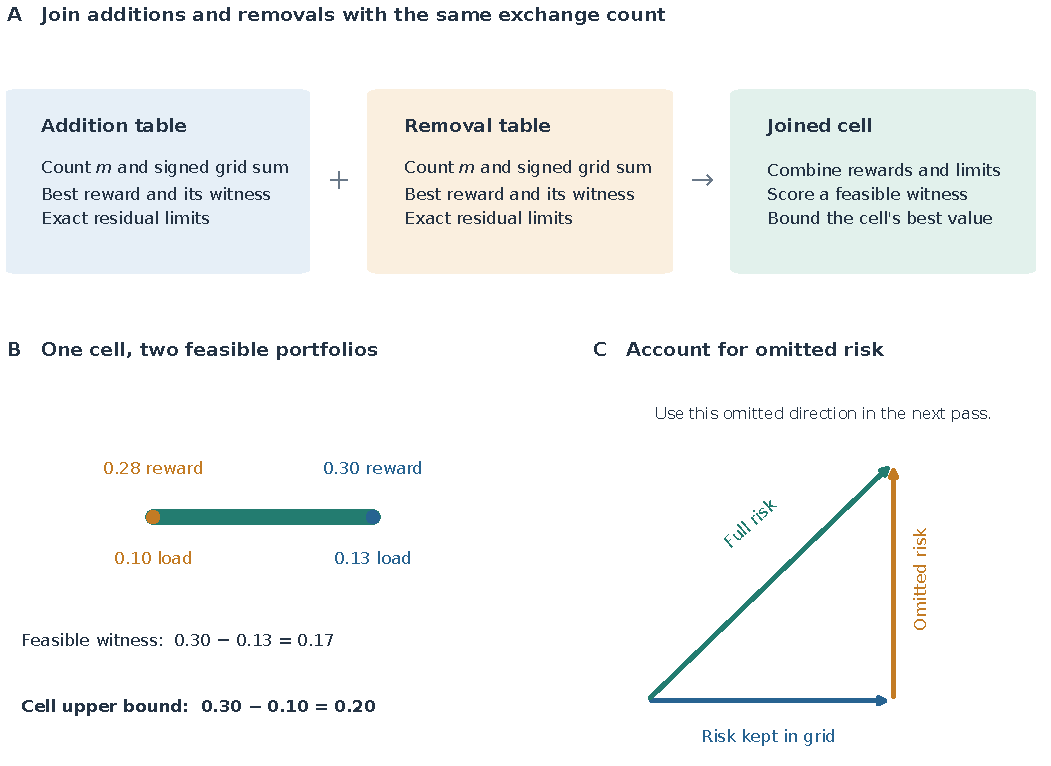
\includegraphics[width=\linewidth]{exchange_grid_algorithm.pdf}
\caption{Exchange-grid algorithm. Panel A shows how addition and removal states are joined. Panel B uses two illustrative portfolios to show how the cell bound is computed. Panel C decomposes the witness's load into the grid projection and the omitted component used to update the next pass.}
\label{fig:grid_algorithm}
\end{figure}

\paragraph{Numerical example.} Panel B of Figure~\ref{fig:grid_algorithm} illustrates how the certificate is constructed.
Suppose two portfolios fall in the same joined cell in a one-factor problem.
Their nominal gains are $0.30$ and $0.28$, and their exact signed risk loadings
are $0.13$ and $0.10$, respectively. With $r=1$, the nominal-gain witness
has objective $0.30-0.13=0.17$. The interval of exact loadings
$[0.10,0.13]$ gives an upper bound of $0.30-0.10=0.20$ for the cell.
The second portfolio actually achieves $0.18$. The bound is valid even
though the highest nominal gain and the smallest risk penalty come from
different portfolios. The solver can retain the first portfolio and the
interval, then use $[0.17,0.20]$ to bound the best objective in the cell.

\paragraph{Additive error and the lattice case.}
If the grid spans all risk directions, the portfolio formed from the two
reward-maximising witnesses in a join has exactly the reward used in
\eqref{eq:grid_bound}. Each coordinate of an item residual lies in an interval of
width $h_j$. The joined box for $m$ exchanges therefore has diameter at most
$2m\|h\|_2$. The norm is 1-Lipschitz, so the gap between \eqref{eq:grid_bound}
and this witness's true objective is at most $2mr\|h\|_2$. Applying this to
a maximising join proves the same additive error bound with
$m\leq\min(q,n-q)$. If the projected loadings lie on the grid, all residuals
vanish. A single count-and-loading recurrence over selected countries then
solves the projected problem exactly. The reference loading is subtracted
at the end. If this grid spans all risk directions, the solution is exact
for the full objective as well.

\subsubsection{Tilting the certificate towards omitted risk}

For a vector $v$ orthogonal to the grid span with $\|v\|_2\leq1$, every portfolio
loading $z=L^\top d$ satisfies
\[
 \|z\|_2 \;\geq\;
    v^\top z+\sqrt{1-\|v\|_2^2}\,\|P^\top z\|_2 .
\]
The right-hand side is the inner product of $z$ with a vector of norm at most
one, obtained by combining $v$ and the unit vector in the direction of its
projection. We can therefore run the same recurrence with the linear rewards
$\mu_i-r a_i^\top v$ and projected radius $r\sqrt{1-\|v\|_2^2}$. Its upper
bound remains valid for the full problem. We set the next tilt to
$(I-PP^\top)z_w/\|z_w\|_2$ using a witness from the preceding maximising join.
The norm inequality is then tight at that witness. The next pass can expose
a different portfolio whose bound is larger. Taking the smallest upper bound
from completed passes and the largest feasible lower bound keeps the certificate
valid. The lower bound always uses full risk, including dimensions omitted
from the grid.

\paragraph{Algorithm.}
Start with zero tilt. Evaluate the exposure reference and the portfolio with
the best nominal gain to initialise the lower bound. The best nominal gain
also gives an upper bound. At each grid resolution:
\begin{enumerate}
 \item Build the two signed tables and join states with the same exchange count.
 \item Find the join with the largest bound in \eqref{eq:grid_bound}, using the
       current adjusted rewards and projected radius. Evaluate its witness
       and any other promising witnesses with full risk.
 \item Keep the best feasible value and the smallest valid upper bound seen
       so far. Stop if their difference meets the tolerance. Otherwise update
       the tilt using the highest-bound join's witness and refine the grid.
\end{enumerate}
If a resource limit interrupts a pass, return the best feasible portfolio
and the bounds from completed passes.

The method has a computational trade-off. For fixed grid dimension, the number
of states grows polynomially in the exchange count and the grid resolution.
Fine or high-dimensional grids can be expensive. The implementation projects
onto at most two directions. It uses a dense recurrence when the projected
loadings lie on a small lattice and otherwise uses sparse signed states.
The early stopping certificate reports the cost of that compression in the
units of the original objective.

\subsubsection{Comparison on discrete and continuous inputs}

We compare against the integer cutting-plane method in
Section~\ref{sec:ellipsoid}. We also disable the tilt as a control. The benchmark
uses 16 instances per synthetic design and reconstructs the fitted objective
for each of the 12 agricultural holdout batches. Timing starts after the
benefits and factor loadings are supplied. The lattice designs give each
factor seven equally spaced levels. The continuous design uses six normally
distributed factor loadings per country. The gap tolerance is $10^{-5}$ in
total-gain units.

\section{Results}\label{sec:results}

\subsection{Heat damages cereal yields}

Table~\ref{tab:firststage} shows that the hottest-month temperature anomaly lowers cereal-yield
growth substantially. With country and year fixed effects, a 1$^{\circ}$C hotter-than-trend
hottest month reduces yield growth by 3.6 percentage points across 155 countries (SE 0.53), and by
2.7 points in emerging and developing economies (SE 0.76). The annual mean anomaly has no
detectable average effect ($-0.61$, SE 1.01), in line with the threshold effects of heat documented
by \citet{schlenker2009}. We report all three shock definitions we examined, because the choice of
the hottest-month anomaly was made after seeing this table. Among countries whose baseline climate
is already hot ($\geq 20^{\circ}$C), the estimate is imprecise ($-0.34$, SE 0.91), so the
first stage is driven mainly by cooler and temperate producers. This matters for interpreting the
allocation rules below.

\begin{table}[t]
\centering
\caption{Heat shocks and cereal-yield growth: first stage}\label{tab:firststage}
\small
\begin{tabular}{lcccc}
\toprule
Sample & Coefficient (SE) & $p$ & Observations & Countries \\
\midrule
All countries & $-3.572$ (0.530) & $<0.001$ & 3,679 & 155 \\
EMDEs & $-2.684$ (0.759) & $<0.001$ & 2,538 & 107 \\
Baseline temp.\ $\geq 20^{\circ}$C & $-0.336$ (0.908) & 0.711 & 1,971 & 83 \\
Annual-mean anomaly as regressor & $-0.612$ (1.006) & 0.543 & 3,679 & 155 \\
\bottomrule
\end{tabular}
\begin{minipage}{0.95\textwidth}\footnotesize\smallskip
\emph{Notes:} Dependent variable: $100\times\Delta\ln$ cereal yield (kg/ha). Regressor: hottest-month
mean temperature minus its 1980--2023 country-specific linear trend ($^{\circ}$C), except in the last
row. Country and year fixed effects; standard errors clustered by country. Observations with
$|\Delta\ln\text{yield}|\geq 1$ are dropped as data errors. The sample is larger than the estimation
sample of Table~\ref{tab:ate}, which also requires the lagged covariates.
\end{minipage}
\end{table}

\subsection{No detectable resilience dividend}

Table~\ref{tab:ate} reports the main estimates for 3,336 country-years in 145 countries. The
median across the 20 sample splits of the average resilience effect is 1.02 percentage points of
yield growth per $^{\circ}$C, with a split-adjusted standard error of 2.12. The 95 per cent
confidence interval, $[-3.13, 5.17]$, is wide. It contains zero, and it also contains effects
larger than the average damage itself. The data therefore cannot distinguish between climate-AI
capability having no effect on heat damage and its offsetting all of it. Other ways of computing
the estimate give the same picture. Using the observation-level median score, the estimate is 0.84
with a country-clustered SE of 1.01, a two-way (country and year) clustered SE of 0.94, or a
Driscoll--Kraay SE of 1.17. Winsorising the scores at the 1st and 99th percentiles gives 0.51
(SE 0.74). The scores are heavy-tailed: the 99th percentile of $|\Gamma|$ is about 300 against a
median of 11.

The average marginal damage implied by the orthogonal scores is similar in the two groups
($-1.49$ with capability and $-1.31$ without, split-adjusted; $-1.52$ overall). That is less than half the fixed-effects estimate on the
same sample ($-3.58$ with country and year effects, and $-3.17$ with year and region effects and the
same covariates; Appendix Table~\ref{tab:recon}). Country fixed effects are therefore not the
reason. The difference arises within the orthogonal estimator, whose scores weight observations by
the inverse of the estimated conditional variance of the shock. We have not been able to reconcile
the two fully, and we treat the scale of the orthogonal estimates with caution.

The classical specification again behaves differently. A two-way fixed-effects regression with a
shock-by-capability interaction gives 0.32 (SE 0.97) for yields. For agricultural value-added growth
it gives 0.82 (SE 0.46, $p\approx0.07$), which would often be reported as weak evidence of a
resilience dividend. The doubly robust estimate for the same outcome is 0.07 (split-adjusted SE
1.01). Once the flexible relationship between capability, income, connectivity and climate is taken
into account, the suggestive interaction disappears, as the Monte Carlo evidence on the interaction
model would lead one to expect.

\begin{table}[t]
\centering
\caption{Resilience effect of climate-AI capability on cereal-yield growth}\label{tab:ate}
\small
\begin{tabular}{lcc}
\toprule
 & Estimate (SE) & 95\% CI \\
\midrule
\multicolumn{3}{l}{\emph{EW-DRPL, average resilience effect}}\\
Median over splits, split-adjusted SE (main) & 1.022 (2.118) & [$-3.13$, 5.17] \\
Observation-level median score, country clusters & 0.843 (1.014) & [$-1.14$, 2.83] \\
\quad two-way clusters (country, year) & 0.843 (0.937) & [$-1.00$, 2.68] \\
\quad Driscoll--Kraay (2 lags) & 0.843 (1.172) & [$-1.46$, 3.14] \\
\quad scores winsorised at 1st/99th percentiles & 0.505 (0.738) & [$-0.94$, 1.95] \\
Split-to-split range & [$-2.56$, 7.47] & \\
\midrule
\multicolumn{3}{l}{\emph{EW-DRPL, mean marginal damage}}\\
Capability ($T=1$, 1,734 obs.) & $-1.489$ (1.188) & [$-3.82$, 0.84] \\
No capability ($T=0$, 1,602 obs.) & $-1.310$ (1.214) & [$-3.69$, 1.07] \\
\midrule
\multicolumn{3}{l}{\emph{Two-way fixed effects (for comparison)}}\\
Heat shock & $-3.386$ (0.820) & \\
Heat shock $\times$ capability & 0.315 (0.970) & \\
Heat shock $\times$ capability, agricultural value added & 0.817 (0.457) & \\
\midrule
\multicolumn{3}{l}{\emph{EW-DRPL, agricultural value added}}\\
Average resilience effect (split-adjusted) & 0.066 (1.014) & [$-1.92$, 2.05] \\
\bottomrule
\end{tabular}
\begin{minipage}{0.95\textwidth}\footnotesize\smallskip
\emph{Notes:} Units: percentage points of annual growth per $^{\circ}$C of hottest-month anomaly.
3,336 country-years in 145 countries (3,305 for agricultural value added). Capability:
climate-AI knowledge stock above the level predicted by income in the previous year. Covariates,
lagged one year: log GDP per capita, internet use, agricultural share, urban share, log population,
log fertiliser use, ND-GAIN readiness and general AI output; also baseline temperature, the
precipitation shock, year and region. Damage rows: split-adjusted SEs.
\end{minipage}
\end{table}

\subsection{Heterogeneity}

Neither the best linear projection of $\Gamma$ on the policy features nor the sorted group effects
reveal a reliable gradient. All six projection coefficients are within 1.4 standard errors of zero,
the largest relative to its SE being inequality ($-1.63$, SE 1.23) and knowledge sovereignty
($-1.58$, SE 1.47). The difference between the top and bottom quintiles of predicted resilience is
4.5 (SE 3.7), and the quintile means are not monotone (Appendix Table~\ref{tab:gates}). The
classification analysis shows that the model predicts the largest resilience effects for
country-years with lower internet use (22 percentage points lower in the top than in the bottom
quintile, SE 4.4), lower knowledge sovereignty and lower income. Because the sorted effects are not
monotone, this describes where the prediction model places resilience rather than where resilience
is. With about 145 countries and noisy scores, the data cannot rank countries by the size of the
resilience dividend.

\subsection{Allocation rules}

Table~\ref{tab:policy} reports the held-out welfare values of the allocation rules for a budget of
30 per cent of the 126 countries with complete distributional data. Values are means over countries
of $\pi(Z_i)B_i(\epsilon)$, which combine the estimated resilience scores with shock size,
population, agricultural exposure and welfare weights.

The table supports three conclusions, and none of them favours data-driven targeting in this
application. First, no rule's value is distinguishable from zero, which is what one would expect
given that the average resilience effect is not. Second, simple rules do at least as well as the
learned trees. Allocating capacity to the poorest 30 per cent of countries has the highest point
value under every $\epsilon>0$, and at $\epsilon=2$ it beats the EW-DRPL tree by 1.39
[$0.02$, $3.26$], the only policy comparison whose interval excludes zero. Third, the rule closest
to building on existing strength, which allocates capacity to the countries with the largest
climate-AI stock, has a value of essentially zero. This is largely mechanical: those countries have
little agricultural exposure and comparatively rich deciles, so even a large resilience effect would
add little equity-weighted welfare. Its difference from the poorest-first rule is not
statistically significant ($-0.65$ [$-1.80$, $0.31$] at $\epsilon=1$).

The equity gain of the $\epsilon=1$ rule over the utilitarian rule is 0.33 [$-0.01$, 0.90] and the
equity price is $-0.06$ [$-0.16$, 0.01]. A negative price, meaning that the equity-weighted rule also
does better on utilitarian welfare, cannot be a property of the population optimum. It reflects the
noise of cross-fitted trees. When the objective counts countries rather than people, every rule's
value is close to zero, and the advantage of poorest-first disappears (Appendix
Table~\ref{tab:unweighted}). The population-weighted results are thus driven by a few populous,
poor and agricultural countries.

The learned trees are readable, but they are not stable. For $\epsilon\le1$ the tree treats 31
countries. Nineteen are low-income countries with a hot baseline climate: eighteen in sub-Saharan Africa
and Myanmar. Twelve have higher incomes and a predominantly domestic climate-AI research base,
including China, India, Indonesia, the Philippines and the United States. At $\epsilon=2$ the root
split moves to internet use, and the low-income branch shrinks to ten countries. Viet Nam is not
treated by any rule; its estimated equity-weighted benefit is slightly negative at $\epsilon=1$
and $\epsilon=2$.
The hot, low-income branch is also the group for which the first stage is weakest
(Table~\ref{tab:firststage}), so its selection reflects exposure and welfare weights more than any
measured resilience effect.

\begin{table}[t]
\centering
\caption{Held-out welfare value of allocation rules (budget $k=0.3$)}\label{tab:policy}
\small
\begin{tabular}{lcccc}
\toprule
Rule & $\epsilon=0$ & $\epsilon=0.5$ & $\epsilon=1$ & $\epsilon=2$ \\
\midrule
EW-DRPL ($\epsilon$-specific tree) & 0.190 & 0.344 & 0.399 & $-0.119$ \\
 & {\footnotesize[$-0.17$, 0.74]} & {\footnotesize[$-0.25$, 1.13]} & {\footnotesize[$-0.40$, 1.30]} & {\footnotesize[$-1.10$, 0.84]} \\
Utilitarian tree & 0.190 & 0.185 & 0.072 & $-0.282$ \\
 & {\footnotesize[$-0.17$, 0.74]} & {\footnotesize[$-0.37$, 0.98]} & {\footnotesize[$-0.69$, 1.01]} & {\footnotesize[$-1.36$, 0.72]} \\
Plug-in tree & 0.387 & 0.284 & 0.475 & 0.789 \\
 & {\footnotesize[$-0.05$, 0.98]} & {\footnotesize[$-0.22$, 1.06]} & {\footnotesize[$-0.19$, 1.37]} & {\footnotesize[$-0.22$, 2.08]} \\
Capable-first & $-0.006$ & $-0.007$ & $-0.007$ & $-0.009$ \\
 & {\footnotesize[$-0.02$, 0.01]} & {\footnotesize[$-0.02$, 0.01]} & {\footnotesize[$-0.04$, 0.02]} & {\footnotesize[$-0.05$, 0.02]} \\
Poorest-first & 0.310 & 0.471 & 0.647 & 1.268 \\
 & {\footnotesize[$-0.08$, 0.89]} & {\footnotesize[$-0.17$, 1.35]} & {\footnotesize[$-0.33$, 1.79]} & {\footnotesize[$-0.62$, 3.26]} \\
Most-agricultural-first & 0.291 & 0.431 & 0.581 & 1.169 \\
 & {\footnotesize[$-0.11$, 0.87]} & {\footnotesize[$-0.21$, 1.30]} & {\footnotesize[$-0.41$, 1.70]} & {\footnotesize[$-0.64$, 3.16]} \\
Random (expected) & 0.130 & 0.176 & 0.213 & 0.358 \\
\midrule
Equity gain $W_\epsilon(\hat\pi_\epsilon)-W_\epsilon(\hat\pi_0)$ & & & 0.327 & 0.164 \\
 & & & {\footnotesize[$-0.01$, 0.90]} & {\footnotesize[$-0.04$, 0.52]} \\
Equity price $W_0(\hat\pi_0)-W_0(\hat\pi_\epsilon)$ & & & $-0.061$ & $-0.020$ \\
 & & & {\footnotesize[$-0.16$, 0.01]} & {\footnotesize[$-0.09$, 0.03]} \\
EW-DRPL minus poorest-first & & & $-0.248$ & $-1.386$ \\
 & & & {\footnotesize[$-0.77$, 0.14]} & {\footnotesize[$-3.26$, $-0.02$]} \\
\bottomrule
\end{tabular}
\begin{minipage}{0.95\textwidth}\footnotesize\smallskip
\emph{Notes:} 126 countries, of which 86 EMDEs; capacity for 37. Each rule is learned on four
country folds and evaluated on the fifth; columns give the inequality aversion used in evaluation.
Values: mean over countries of $\pi(Z_i)B_i(\epsilon)$, where $B_i$ includes the shock size, the
population scale and the agricultural exposure of each decile (allocated to the lowest deciles
first). 95 per cent country-cluster bootstrap intervals in brackets (500 replications), holding the
learned rules fixed. Capable-first: largest climate-AI stock per capita; poorest-first: lowest GDP
per capita; most-agricultural-first: highest agricultural employment share. Trees treat fewer than
37 countries because a depth-2 tree can only treat whole leaves.
\end{minipage}
\end{table}

\subsection{Robustness}\label{sec:robust}

Table~\ref{tab:sens} reports alternative specifications. The average resilience effect stays
imprecise and close to zero relative to its standard error when the non-orthogonal score is used,
when propensity scores are clipped at $[0.05,0.95]$, with random-forest nuisance models, in the EMDE
subsample, with the capability indicator that is not adjusted for income, and for agricultural value
added. The exception is the annual-mean anomaly, for which the estimate is $-5.59$ (SE 1.92). The
annual anomaly has no first-stage effect on yields on average (Table~\ref{tab:firststage}), so this
estimate compares sensitivities that are both close to zero. It is nevertheless the one
specification in which capability is associated with significantly greater sensitivity, and we
report it as such.

The allocation rules are much less stable than the average effect. Relative to the main rules, the
treated sets are unchanged under alternative clipping, and at $\epsilon=2$ also under uniform
exposure. Under the other specifications they overlap only partly, with Jaccard indices between
0.02 and 0.71 at $\epsilon=1$ and between 0.08 and 0.51 at $\epsilon=2$. With a budget of 20 per
cent, the held-out values of the learned rules lie between $-0.28$ and 0.08. This instability is the empirical
counterpart of the small-sample regret documented in the Monte Carlo study, and it is why we do not
draw country-specific recommendations from the trees.

\begin{table}[t]
\centering
\caption{Sensitivity analysis}\label{tab:sens}
\small
\resizebox{\textwidth}{!}{%
\begin{tabular}{lccccc}
\toprule
 & & & \multicolumn{3}{c}{Treated set vs main} \\
\cmidrule(lr){4-6}
Specification & Obs. & Average effect (SE) & $n$ ($\epsilon=1$) & Jaccard ($\epsilon=1$) & Jaccard ($\epsilon=2$) \\
\midrule
Main & 3,336 & 0.843 (1.014) & 31 & 1.00 & 1.00 \\
(a) Non-orthogonal slope score & 3,336 & 0.727 (1.126) & 22 & 0.71 & 0.51 \\
(b) Clipping at $[0.05,0.95]$ & 3,336 & 0.978 (1.070) & 31 & 1.00 & 1.00 \\
(c) Annual-mean anomaly as shock & 3,336 & $-5.594$ (1.916) & 33 & 0.21 & 0.11 \\
(d) Random-forest nuisance models & 3,336 & $-0.138$ (0.760) & 22 & 0.71 & 0.42 \\
(e) EMDEs only & 2,247 & 0.669 (1.417) & 25 & 0.51 & 0.28 \\
(f) Capability without income adjustment & 3,336 & 2.258 (1.672) & 33 & 0.14 & 0.09 \\
(g) Agricultural value added as outcome & 3,305 & 0.001 (0.610) & 26 & 0.02 & 0.08 \\
(h) Uniform exposure across deciles & -- & -- & 22 & 0.71 & 1.00 \\
\bottomrule
\end{tabular}}
\begin{minipage}{0.95\textwidth}\footnotesize\smallskip
\emph{Notes:} Average effect: observation-level median score over 20 splits, country-clustered SE.
$n$: number of countries treated by the full-sample $\epsilon=1$ tree. Jaccard: overlap with the
main treated set.
\end{minipage}
\end{table}

\subsection{Decile incomes, aggregate growth and the cost of AI}\label{sec:res_decile}

We also applied EW-DRPL directly to decile income growth from 1,334 household-survey spells in 124
countries, and to GDP per capita growth (Appendix~\ref{app:decile}). Neither has a usable first
stage. The annual temperature anomaly has no detectable effect on GDP growth in our 1998--2023
sample ($-0.10$, SE 0.18), even in hot EMDEs ($-0.27$, SE 0.46), and spell-averaged anomalies have
none on decile growth. Without measurable damage there is nothing for capability to reduce, and the
resulting resilience estimates are uninformative.

On the cost side, double machine learning estimates of the association between the climate-AI
knowledge stock and per-capita electricity use ($-0.015$, SE 0.112) and CO$_2$ emissions (0.061,
SE 0.099), and between general AI output and the same outcomes (0.070, SE 0.060, and 0.028, SE
0.056), are imprecise and centred near zero. These intervals do not rule out economically meaningful
effects, but they give no indication that national AI research capacity drives economy-wide energy
demand. The electricity footprint documented by \citet{iea2025} arises where data centres are
located, which is not necessarily where AI research is produced.

\section{Monte Carlo evidence}\label{sec:mc}

Before turning to the data, we examine how EW-DRPL performs at sample sizes typical of
cross-country work, where the asymptotics behind Proposition~\ref{prop:regret} may be a poor guide.

\paragraph{Design.} Each simulated country has six correlated characteristics that mimic log income,
inequality, internet access, agricultural share, baseline temperature and knowledge sovereignty.
It is observed in $J=4$ spells, each with ten deciles. Capability is assigned with probability
$\mathrm{logit}^{-1}(1.5\,\text{income}+0.5\,\text{internet})$, so it is strongly confounded with
development, as in the data. Shocks are normal with a variance that rises with the agricultural
share. Shock sensitivity is
$\beta_d=-(1+0.5\,\text{agri}-0.1d)+T\,\rho_d(X)$, with resilience effect
$\rho_d(X)=0.8(1-d/10)\,\mathbf 1\{\text{internet}>0\}$. Capability therefore protects the poorer
deciles more, and only in connected countries. Income levels depend non-linearly on the
covariates and on $T$, so capability is also correlated with growth itself. Decile incomes are
log-normal with a spread that increases with inequality. We draw $N=150$ and $N=500$ countries,
set the budget at $k=0.3$ and run 200 replications. For every replication we compute the best
depth-2 tree under the true benefits, the oracle, and measure each method's regret against it
under the $\epsilon$-weighted welfare criterion.

\paragraph{Comparators.} EW-DRPL learns the tree from the equity-weighted orthogonal scores. The
utilitarian rule learns it from $\epsilon=0$ scores and is evaluated under $\epsilon$. The plug-in
rule uses $\hat m_{d,1}-\hat m_{d,0}$ without the doubly robust correction. The IPW-only rule drops
the outcome model. The raw-score rule uses the non-orthogonalised slope signal $\psi_d$ in place of
$\psi^*_d$. The naive rule ranks countries by the fitted interaction effects from a pooled
regression of $Y$ on $S$, $S\times T$ and $S\times T\times Z$ with decile fixed effects, the
standard specification in the applied literature.

\begin{table}[t]
\centering
\caption{Monte Carlo results}\label{tab:mc}
\scriptsize
\resizebox{\textwidth}{!}{% Monte Carlo summary for EW-DRPL. Requires \usepackage{booktabs}.
% Cells: mean (MC standard error) over 200 replications.
\begin{tabular}{lcccccc}
\toprule
 & \multicolumn{3}{c}{$N=150$} & \multicolumn{3}{c}{$N=500$} \\
\cmidrule(lr){2-4}\cmidrule(lr){5-7}
Method & $\varepsilon=0$ & $\varepsilon=1$ & $\varepsilon=2$ & $\varepsilon=0$ & $\varepsilon=1$ & $\varepsilon=2$ \\
\midrule
\multicolumn{7}{l}{\emph{Panel A: regret vs.\ oracle tree (true welfare)}} \\
EW-DRPL & 0.058 (0.002) & 0.070 (0.002) & 0.070 (0.005) & 0.028 (0.001) & 0.047 (0.002) & 0.051 (0.003) \\
EW-DRPL-crossfit & 0.057 (0.001) & 0.073 (0.002) & 0.079 (0.005) & 0.032 (0.001) & 0.050 (0.002) & 0.056 (0.003) \\
Utilitarian-DR & 0.058 (0.002) & 0.078 (0.002) & 0.106 (0.008) & 0.028 (0.001) & 0.052 (0.002) & 0.085 (0.007) \\
Plug-in & 0.046 (0.002) & 0.062 (0.002) & 0.069 (0.007) & 0.027 (0.001) & 0.043 (0.002) & 0.048 (0.004) \\
IPW-only & 0.064 (0.001) & 0.076 (0.002) & 0.074 (0.006) & 0.053 (0.001) & 0.075 (0.001) & 0.077 (0.005) \\
Raw-psi-DR & 0.066 (0.001) & 0.078 (0.002) & 0.083 (0.006) & 0.050 (0.001) & 0.069 (0.002) & 0.084 (0.006) \\
Naive-TWFE & 0.078 (0.001) & 0.105 (0.002) & 0.156 (0.009) & 0.077 (0.000) & 0.106 (0.001) & 0.166 (0.008) \\
Oracle & 0.000 (0.000) & 0.000 (0.000) & 0.000 (0.000) & 0.000 (0.000) & 0.000 (0.000) & 0.000 (0.000) \\
\midrule
\multicolumn{7}{l}{\emph{Panel B: share of oracle-treated countries recovered}} \\
EW-DRPL & 0.393 (0.010) & 0.376 (0.011) & 0.355 (0.009) & 0.584 (0.010) & 0.505 (0.013) & 0.419 (0.011) \\
EW-DRPL-crossfit & 0.405 (0.009) & 0.368 (0.009) & 0.355 (0.008) & 0.556 (0.008) & 0.488 (0.010) & 0.408 (0.008) \\
Utilitarian-DR & 0.393 (0.010) & 0.351 (0.010) & 0.336 (0.010) & 0.584 (0.010) & 0.467 (0.010) & 0.454 (0.010) \\
Plug-in & 0.478 (0.012) & 0.422 (0.011) & 0.396 (0.010) & 0.619 (0.012) & 0.532 (0.014) & 0.454 (0.013) \\
IPW-only & 0.363 (0.009) & 0.330 (0.010) & 0.321 (0.008) & 0.420 (0.008) & 0.332 (0.008) & 0.293 (0.008) \\
Raw-psi-DR & 0.349 (0.009) & 0.334 (0.009) & 0.326 (0.009) & 0.435 (0.009) & 0.373 (0.010) & 0.338 (0.009) \\
Naive-TWFE & 0.118 (0.006) & 0.325 (0.005) & 0.327 (0.004) & 0.093 (0.005) & 0.342 (0.003) & 0.338 (0.003) \\
Oracle & 1.000 (0.000) & 1.000 (0.000) & 1.000 (0.000) & 1.000 (0.000) & 1.000 (0.000) & 1.000 (0.000) \\
\midrule
\multicolumn{7}{l}{\emph{Panel C: ATE of $\rho$ (average over countries and deciles): bias (MC SE) and RMSE}} \\
ATE-DR & -0.057 (0.076) & 1.075 &  & 0.010 (0.005) & 0.072 &  \\
ATE-DR-raw & 0.052 (0.034) & 0.477 &  & -0.000 (0.006) & 0.086 &  \\
ATE-plugin & 0.036 (0.023) & 0.330 &  & 0.011 (0.005) & 0.069 &  \\
ATE-IPW & 0.077 (0.037) & 0.526 &  & 0.022 (0.006) & 0.084 &  \\
ATE-naive & 0.291 (0.006) & 0.303 &  & 0.300 (0.003) & 0.303 &  \\
\bottomrule
\end{tabular}
}
\begin{minipage}{\textwidth}\footnotesize\smallskip
\emph{Notes:} 200 replications; Monte Carlo standard errors in parentheses. Regret is the
difference between the welfare of the oracle depth-2 tree and that of the learned rule, both
evaluated with the true benefits under the indicated inequality aversion $\epsilon$. Budget
$k=0.3$. ``crossfit'' learns the tree on four country folds and applies it to the fifth.
Propensity scores are clipped to $[0.1,0.9]$.
\end{minipage}
\end{table}

\paragraph{Results.} Table~\ref{tab:mc} and Appendix Figure~\ref{fig:regret} report the results.
Four findings stand out.

First, the standard interaction regression is a poor targeting device. Its regret exceeds that of
EW-DRPL in every cell of the design, by between 30 per cent ($N=150$, $\epsilon=0$) and 71 per cent
($N=500$, $\epsilon=2$). At $\epsilon=0$ it recovers only about a tenth of the countries the oracle
would treat, fewer than random allocation would. Its implied average resilience effect is biased
upward by about 0.30, against a true average of about 0.18, because a pooled interaction model
cannot separate capability from the characteristics it is correlated with.

Second, equity weighting matters when the planner is strongly inequality averse. At $\epsilon=2$
the utilitarian rule's regret is 0.104 at $N=150$ and 0.084 at $N=500$, against 0.067 and 0.048 for
EW-DRPL, reductions of 35 and 43 per cent. At $\epsilon=1$ the reduction is smaller (9 and 15 per
cent), and at $\epsilon=0$ the two rules coincide by construction.

Third, orthogonalisation improves targeting and, in larger samples, estimation. Replacing
$\psi^*_d$ by the raw Robinson signal raises regret at $N=500$ by 0.019 to 0.033 and the RMSE of
the average resilience effect from 0.065 to 0.082. At $N=150$, however, the orthogonal score has
the larger RMSE (0.56 against 0.36), because the correction terms divide by estimated propensities
and shock variances. Dropping the outcome model (IPW-only) raises regret in every cell.

Fourth, the doubly robust correction does not improve targeting over a well-specified plug-in rule
in this design. The plug-in rule, which ranks countries by $\hat m_{d,1}-\hat m_{d,0}$, has lower
regret at $N=150$, the same regret at $N=500$, and a lower RMSE for the average effect at $N=150$ (0.33 against 0.56). Its
advantage is variance: it omits the inverse-weighted corrections. The doubly robust rule is
insurance against misspecification of the slope model, which our design does not impose. We
therefore report both in the application. Clipping the propensity score at $[0.1,0.9]$ rather than
$[0.05,0.95]$ cuts the RMSE of the doubly robust average effect at $N=150$ from 1.08 to 0.56 and
leaves regret essentially unchanged (Appendix Table~\ref{tab:mc_trim}).

The design is favourable to the estimator in several respects. Shocks are normal and independent
across countries, the response is linear in the shock, capability is redrawn for every spell, and
exposure and shock sizes are known. The application departs from each of these. The practical
lesson for cross-country work with around 150 countries is that average effects will be estimated
imprecisely even when targeting rules are informative, and that limited overlap between countries
with and without capability is the binding constraint.

\subsection{Budget-neutral swaps in simulations and agricultural data}\label{res:swaps}

Appendix Table~\ref{tab:swap_simulation} compares policies over 500 replications for each simulation
design. Under weak overlap and heterogeneous effects, robust swaps lose to the exposure
reference in 29.0 per cent of test samples, compared with 40.6 per cent for DR swaps and
35.8 per cent for plug-in swaps. Their mean gain is 0.0096, compared with 0.0053 and 0.0078.
The paired mean gains of robust over DR and plug-in are 0.0044 (Monte Carlo SE 0.0010)
and 0.0018 (SE 0.0009), respectively. Mean-score swaps lose in 36.2 per cent of
weak-overlap draws. The paired gain of robust over mean-score swaps is 0.0016
(SE 0.0009). The mean-gain comparisons with plug-in and mean-score swaps are small
relative to their Monte Carlo uncertainty. Under moderate overlap, mean-score swaps
have a slightly lower loss rate than robust swaps (26.8 against 27.2 per cent).
When effects are homogeneous, all fitted methods have negative mean gains. Robust
swaps underperform the exposure reference in 87.0 per cent of these replications.

In the five country folds, robust swaps replace 21 of 37 places and have an estimated
gain of 0.455 (conditional 95 per cent interval $[-0.122,1.219]$). With 0.05 clipping
in the evaluation score, the estimate is 0.432 ($[-0.147,1.187]$). Holding out entire
regions changes which countries are compared and which model is used to score them.
The robust rule replaces 14 of 37 places and has an estimated gain of 0.065
($[-0.184,0.403]$), or 0.067 ($[-0.175,0.399]$) with the alternative clipping.
DR, plug-in and mean-score swaps have higher point estimates in the regional
exercise. In the country folds their point estimates are all at or below zero.
The comparisons give no reliable evidence that robust swaps improve on the
exposure ranking in the agricultural sample. They do demonstrate that model choice
and the comparison population can change the assessment even under an exact quota.

\subsection{Ellipsoidal portfolio risk and held-out welfare}\label{res:ellipsoid}

Figure~\ref{fig:simulation_tradeoff} reports results from 600 independent test evaluations.
Under weak overlap, the ellipsoidal portfolio loses to the reference in 3.5 per
cent of replications, against 26.5 per cent for threshold swaps and 22.5 per cent
for ranking the pooled means. Its paired average gain over threshold swaps is
0.00527 (Monte Carlo SE 0.00137). Its mean gain is virtually the same as that
of the pooled-mean rule. With moderate overlap, paying for protection reduces
mean gain by 0.00448 relative to pooling alone (SE 0.00137) and lowers the loss
rate from 18.5 to 5.0 per cent. When the true effects are homogeneous the
reference is optimal. The penalty reduces mean losses from 0.0206 under the
pooled-mean policy to 0.0021, and reduces but does not eliminate the risk of
making unnecessary exchanges.

\begin{figure}[htbp]
\centering
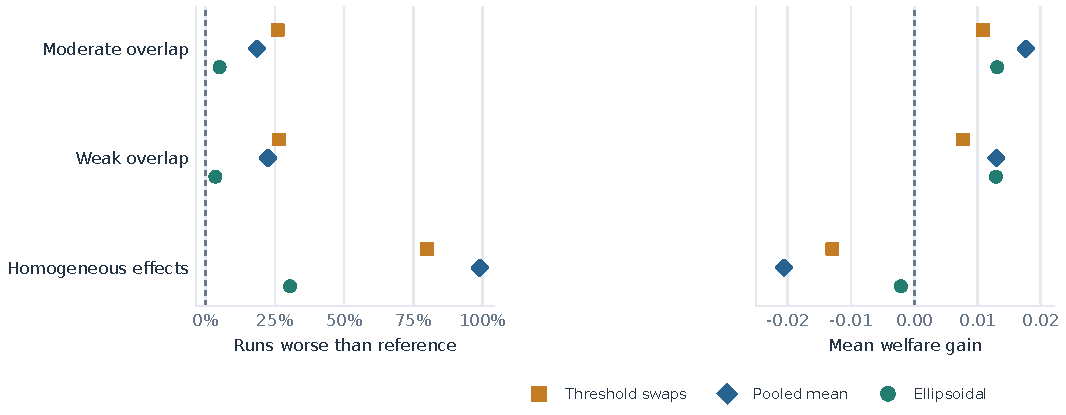
\includegraphics[width=\linewidth]{simulation_tradeoff.pdf}
\caption{Risk and mean welfare in the ellipsoidal portfolio simulations, using 200 replications per design. A loss occurs when a policy underperforms the exposure reference. Both measures are relative to that reference, which has zero gain and zero loss rate by construction. See Appendix Table~\ref{tab:ellipsoid_simulation} for full results.}
\label{fig:simulation_tradeoff}
\end{figure}

The solver reaches the stated total-gain tolerance of $10^{-5}$ in 591 of the
600 simulations under finite solve limits. Across all replications the worst
remaining gap in mean gain per test country is below $0.00082$. All 12
agricultural batches reach the tolerance. Their largest remaining gap in
mean gain per country is approximately $1.1\times10^{-7}$.

In held-out country folds the ellipsoidal portfolio replaces seven places and
has an estimated gain of $-0.271$ (conditional 95 per cent interval
$[-0.754,-0.009]$, Figure~\ref{fig:heldout_welfare}). The estimate is
$-0.256$ with propensity clipping at 0.05. For whole-region holdouts it retains
the reference in every batch. The small solver gaps rule out incomplete
numerical optimisation as an explanation for weak held-out welfare. The
ellipsoid represents uncertainty in fitted changes in heat sensitivity. It
does not resolve the limitations of the research proxy, prediction across
regions, or the uncertainty of using the data to choose a portfolio. The
simulation results show a risk--return trade-off in the specified designs.
The application gives little reason to change an exposure-based ranking
on the available evidence.

\begin{figure}[htbp]
\centering
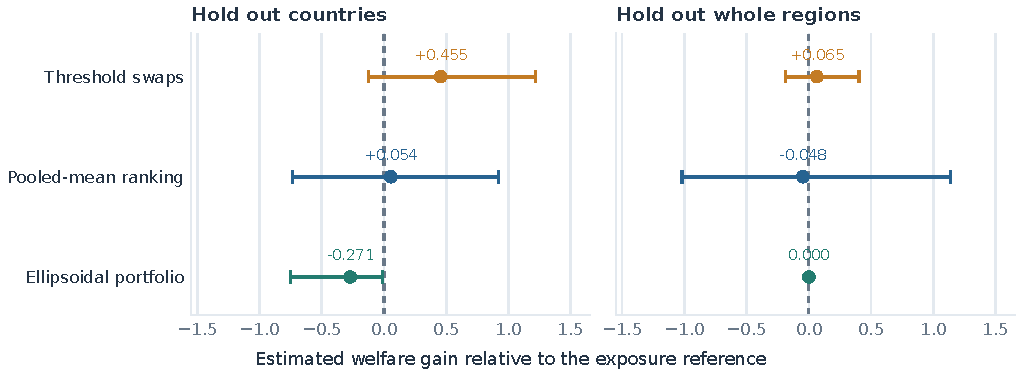
\includegraphics[width=\linewidth]{heldout_welfare.pdf}
\caption{Estimated welfare gains over the exposure reference on held-out countries and whole regions. Each method allocates exactly 37 places. Bars show conditional bootstrap 95\% intervals with the fitted rules and scores held fixed. The ellipsoidal rule retains the reference in the region folds, so its gain and interval are zero by construction. See Appendix Table~\ref{tab:ellipsoid_application} for numerical results.}
\label{fig:heldout_welfare}
\end{figure}

\subsection{Exchange-grid solver benchmark}\label{res:exchange_grid}

\begin{figure}[htbp]
\centering
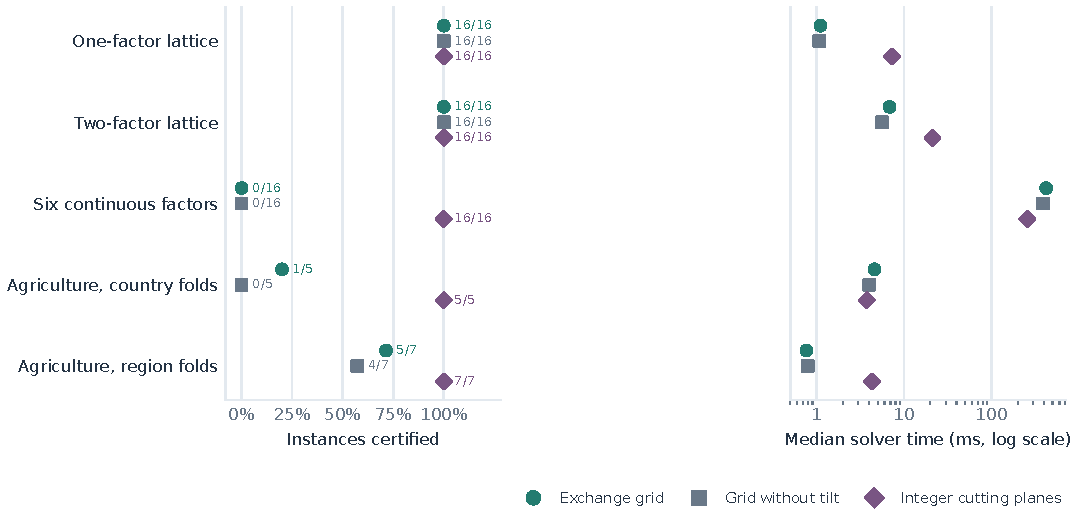
\includegraphics[width=\linewidth]{solver_benchmark.pdf}
\caption{Solver certificates and median runtime across five designs. Fractions in the left panel show the number of instances meeting the total-gain gap tolerance of $10^{-5}$. The right panel reports milliseconds on a log scale for all instances, including runs that stop before certification. Times are specific to this machine. See Appendix Table~\ref{tab:exchange_grid} for the counts.}
\label{fig:solver_benchmark}
\end{figure}

On the one- and two-factor lattices the exchange-grid method certifies every
instance and attains the same objective as the integer cutting-plane solver.
Its median runtime is about one sixth and one third of that solver's,
respectively, on this machine. Both grid variants use the same exact
recurrence on these inputs. The speed comparisons therefore measure the
benefit of the lattice recurrence. Neither grid variant closes the gap on the
six-continuous-factor design. The tilt comparison isolates the benefit of
accounting for omitted directions. The median gap falls from 3.811 to 3.300,
while integer cutting planes certify every instance. On the
agricultural objectives the tilted grid certifies six of 12 batches, against
four for the untilted grid and 12 for integer cutting planes. The new
recurrence is competitive on small discrete risk signatures. Integer cutting
planes provide stronger certificates on the fitted agricultural problems,
so the agricultural welfare comparisons in Section~\ref{res:ellipsoid}
continue to use those solutions.

\section{Discussion and policy implications}\label{sec:discussion}

\paragraph{Who benefits?} The special issue asks who benefits from AI-driven climate solutions. Our
answer for agriculture, the sector in which heat reaches the poor most directly, is that the
benefit is not yet visible in aggregate outcomes. Countries whose climate-AI research capacity
exceeds what their income would predict suffer the same yield losses from hot months as other
countries. This does not mean that AI-based adaptation tools fail where they are deployed. It means
that national research capacity, the most widely available measure of AI capability, has not
translated into economy-wide resilience large enough to detect, and that claims about AI's
contribution to adaptation should be judged against measured damages rather than technical
potential. The finding is consistent with \citet{larosa2024}, who argue that AI helps vulnerable
communities only when it is accessible to them. Research output that remains in universities, or
that is produced mainly by foreign partners, may not reach the extension services, insurers and
farmers through whom resilience would be built.

\paragraph{Under what conditions?} The heterogeneity estimates are imprecise, but their pattern is
informative for policy design. The coefficient on inequality suggests that capability is, if
anything, less protective in more unequal countries, mirroring the finding of \citet{dong2024}
that inequality weakens AI's carbon-abatement benefits. The learned allocation rules, although unstable across specifications, repeatedly
select on two conditions, connectivity and knowledge sovereignty, rather than on income or existing
AI strength. Poorly connected countries in hot climates, where yield damages are large and
agricultural exposure is high, appear in every rule. Where connectivity is higher, the rules favour
countries whose climate-AI research is predominantly domestic. Both conditions point to the same
policy lever: AI capacity yields resilience only if it is embedded in local institutions and if
the people exposed to heat can be reached.

\paragraph{Who bears the costs?} The economy-wide energy and emissions footprint of national AI
research capacity is too small to detect. This is not evidence that AI is environmentally benign.
The electricity and water demands of AI arise in data centres \citep{iea2025,devries2023}, which are
concentrated in a few, mostly high-income locations, and the countries that build research capacity
for adaptation are not those that host the infrastructure. The distributional question on the cost
side is therefore a cross-border one, between the places that bear the environmental footprint of
AI infrastructure and the places that might benefit from AI-enabled adaptation. It cannot be
answered with national research indicators.

\paragraph{Implications for emerging and developing economies.} Three implications follow for
governments and development partners in emerging and developing economies, including Viet Nam and
its ASEAN neighbours. First, the most common allocation heuristic, building on existing strength,
performs worst in our evaluation. Concentrating capacity where climate-AI research is already
strongest yields almost no equity-weighted resilience, because those countries have little
agricultural exposure. Second, programmes should be evaluated against measured damages. The
method in this paper can be applied to programme-level or subnational data, where both damages
and capability are measured more precisely than in cross-country aggregates. Third, the choice of
inequality aversion is a political decision that our framework makes explicit. In our application
it changes the recommended set of countries only at high values of $\epsilon$. At $\epsilon=2$ the
rule includes Viet Nam and four other ASEAN members, because the region combines high exposure of
lower-income rural households to heat with modest domestic climate-AI research. For Viet Nam, where
agriculture remains an important source of income for poorer rural households, the result supports investment in domestically led applied
climate-AI, such as agro-advisory and early-warning services, rather than in research output as
such.

\paragraph{Limitations.} Four limitations qualify these conclusions. First, bibliometric output
measures research capacity, not deployment. A direct measure of AI use in agriculture and disaster
management would sharpen the estimates considerably, and no such measure currently exists across
countries. Second, overlap between countries with and without income-adjusted capability is
limited, and about half of country-years have propensity scores outside $[0.1,0.9]$. This is a
property of the data, not of the estimator, but it limits precision. Third, identification of the
resilience effect rests on selection on observables for shock sensitivity
(Assumption~\ref{as:select}). Unobserved factors that raise both research capacity and agricultural
resilience, such as strong agricultural research institutes, could bias the estimates in either
direction. Fourth, the decile exposure of agricultural income is approximated from employment
shares. Household-survey data on income sources by decile would allow a direct measure.

\section{Conclusion}\label{sec:conclusion}

This paper set out to answer a planner's question: if climate-AI capacity can be built in only some
countries, where should it go first when the welfare of the poor counts for more? We developed
equity-weighted doubly robust policy learning to answer it. The method combines exogenous
temperature shocks, orthogonal doubly robust scores for the effect of capability on shock
sensitivity, Atkinson welfare weights over income deciles, and interpretable allocation rules
learned under a budget. We established its regret properties and showed in simulations that it
outperforms the interaction regressions common in the applied literature by a wide margin. Equity
weighting matters most when inequality aversion is high, and orthogonalisation matters for
reliable targeting.

Applied to cereal yields in 145 countries, the method finds strong heat damages but no detectable
resilience dividend from climate-AI research capacity. The estimates rule out effects larger than
about two-thirds of the damage. The allocation most often used in practice, building on existing
AI strength, delivers essentially no equity-weighted benefit, while rules that prioritise the poorest and the most
agriculturally dependent countries have higher, though imprecise, value. Inequality aversion changes the recommended
allocation only when it is high, at which point Viet Nam and most of its ASEAN neighbours enter the
priority set.

The broader lesson for research on AI, climate change and inclusive development is methodological
as well as substantive. Questions about who benefits are questions about targeting under
heterogeneity, and they call for methods that estimate allocation rules and their welfare
consequences directly. They also call for better data. The binding constraints in our application
are the absence of cross-country measures of AI deployment and the limited overlap between countries
with and without capability. Programme-level and subnational data on AI-enabled adaptation services
would allow the same method to deliver much sharper answers. The code is released with the paper
for that purpose.

\section*{Declarations}

\paragraph{Data availability.} All data are publicly available from the sources cited in
Section~\ref{sec:data}. The code that downloads the data, builds the panels and reproduces every
table and figure, including the EW-DRPL package and the Monte Carlo study, will be deposited in a
public repository on publication. OpenAlex counts were retrieved on 27 November 2026.

\paragraph{Funding.} The author received no funding for this research.

\paragraph{Competing interests.} The author declares no competing interests.


\bibliographystyle{plainnat}
\bibliography{references}

\clearpage
\appendix
\section{Additional Monte Carlo results}\label{app:mc}

\begin{table}[t]
\centering
\caption{Monte Carlo results}\label{tab:mc}
\scriptsize
\resizebox{\textwidth}{!}{% Monte Carlo summary for EW-DRPL. Requires \usepackage{booktabs}.
% Cells: mean (MC standard error) over 200 replications.
\begin{tabular}{lcccccc}
\toprule
 & \multicolumn{3}{c}{$N=150$} & \multicolumn{3}{c}{$N=500$} \\
\cmidrule(lr){2-4}\cmidrule(lr){5-7}
Method & $\varepsilon=0$ & $\varepsilon=1$ & $\varepsilon=2$ & $\varepsilon=0$ & $\varepsilon=1$ & $\varepsilon=2$ \\
\midrule
\multicolumn{7}{l}{\emph{Panel A: regret vs.\ oracle tree (true welfare)}} \\
EW-DRPL & 0.058 (0.002) & 0.070 (0.002) & 0.070 (0.005) & 0.028 (0.001) & 0.047 (0.002) & 0.051 (0.003) \\
EW-DRPL-crossfit & 0.057 (0.001) & 0.073 (0.002) & 0.079 (0.005) & 0.032 (0.001) & 0.050 (0.002) & 0.056 (0.003) \\
Utilitarian-DR & 0.058 (0.002) & 0.078 (0.002) & 0.106 (0.008) & 0.028 (0.001) & 0.052 (0.002) & 0.085 (0.007) \\
Plug-in & 0.046 (0.002) & 0.062 (0.002) & 0.069 (0.007) & 0.027 (0.001) & 0.043 (0.002) & 0.048 (0.004) \\
IPW-only & 0.064 (0.001) & 0.076 (0.002) & 0.074 (0.006) & 0.053 (0.001) & 0.075 (0.001) & 0.077 (0.005) \\
Raw-psi-DR & 0.066 (0.001) & 0.078 (0.002) & 0.083 (0.006) & 0.050 (0.001) & 0.069 (0.002) & 0.084 (0.006) \\
Naive-TWFE & 0.078 (0.001) & 0.105 (0.002) & 0.156 (0.009) & 0.077 (0.000) & 0.106 (0.001) & 0.166 (0.008) \\
Oracle & 0.000 (0.000) & 0.000 (0.000) & 0.000 (0.000) & 0.000 (0.000) & 0.000 (0.000) & 0.000 (0.000) \\
\midrule
\multicolumn{7}{l}{\emph{Panel B: share of oracle-treated countries recovered}} \\
EW-DRPL & 0.393 (0.010) & 0.376 (0.011) & 0.355 (0.009) & 0.584 (0.010) & 0.505 (0.013) & 0.419 (0.011) \\
EW-DRPL-crossfit & 0.405 (0.009) & 0.368 (0.009) & 0.355 (0.008) & 0.556 (0.008) & 0.488 (0.010) & 0.408 (0.008) \\
Utilitarian-DR & 0.393 (0.010) & 0.351 (0.010) & 0.336 (0.010) & 0.584 (0.010) & 0.467 (0.010) & 0.454 (0.010) \\
Plug-in & 0.478 (0.012) & 0.422 (0.011) & 0.396 (0.010) & 0.619 (0.012) & 0.532 (0.014) & 0.454 (0.013) \\
IPW-only & 0.363 (0.009) & 0.330 (0.010) & 0.321 (0.008) & 0.420 (0.008) & 0.332 (0.008) & 0.293 (0.008) \\
Raw-psi-DR & 0.349 (0.009) & 0.334 (0.009) & 0.326 (0.009) & 0.435 (0.009) & 0.373 (0.010) & 0.338 (0.009) \\
Naive-TWFE & 0.118 (0.006) & 0.325 (0.005) & 0.327 (0.004) & 0.093 (0.005) & 0.342 (0.003) & 0.338 (0.003) \\
Oracle & 1.000 (0.000) & 1.000 (0.000) & 1.000 (0.000) & 1.000 (0.000) & 1.000 (0.000) & 1.000 (0.000) \\
\midrule
\multicolumn{7}{l}{\emph{Panel C: ATE of $\rho$ (average over countries and deciles): bias (MC SE) and RMSE}} \\
ATE-DR & -0.057 (0.076) & 1.075 &  & 0.010 (0.005) & 0.072 &  \\
ATE-DR-raw & 0.052 (0.034) & 0.477 &  & -0.000 (0.006) & 0.086 &  \\
ATE-plugin & 0.036 (0.023) & 0.330 &  & 0.011 (0.005) & 0.069 &  \\
ATE-IPW & 0.077 (0.037) & 0.526 &  & 0.022 (0.006) & 0.084 &  \\
ATE-naive & 0.291 (0.006) & 0.303 &  & 0.300 (0.003) & 0.303 &  \\
\bottomrule
\end{tabular}
}
\begin{minipage}{\textwidth}\footnotesize\smallskip
\emph{Notes:} 200 replications; Monte Carlo standard errors in parentheses. Regret is the
difference between the welfare of the oracle depth-2 tree and that of the learned rule, both
evaluated with the true benefits under the indicated inequality aversion $\epsilon$. Budget
$k=0.3$. ``crossfit'' learns the tree on four country folds and applies it to the fifth.
Propensity scores are clipped to $[0.1,0.9]$.
\end{minipage}
\end{table}

\begin{table}[htbp]
\centering
\caption{Monte Carlo: propensity trimming and the doubly robust estimator}\label{tab:mc_trim}
\small
\begin{tabular}{lcccccc}
\toprule
 & & \multicolumn{2}{c}{Average effect} & \multicolumn{3}{c}{EW-DRPL regret} \\
\cmidrule(lr){3-4}\cmidrule(lr){5-7}
Trimming & $N$ & Bias & RMSE & $\epsilon=0$ & $\epsilon=1$ & $\epsilon=2$ \\
\midrule
$[0.05,0.95]$ & 150 & -0.057 & 1.075 & 0.058 & 0.070 & 0.070 \\
$[0.05,0.95]$ & 500 & 0.010 & 0.072 & 0.028 & 0.047 & 0.051 \\
$[0.1,0.9]$ & 150 & -0.012 & 0.559 & 0.055 & 0.068 & 0.067 \\
$[0.1,0.9]$ & 500 & 0.011 & 0.065 & 0.027 & 0.044 & 0.048 \\
\bottomrule
\end{tabular}
\begin{minipage}{0.95\textwidth}\footnotesize\smallskip
\emph{Notes:} 200 replications of the design in Section~\ref{sec:mc} under each trimming rule.
\end{minipage}
\end{table}


\section{Additional results for cereal yields}\label{app:agri}

\begin{table}[t]
\centering
\caption{Heat shocks and cereal-yield growth: first stage}\label{tab:firststage}
\small
\begin{tabular}{lcccc}
\toprule
Sample & Coefficient (SE) & $p$ & Observations & Countries \\
\midrule
All countries & $-3.572$ (0.530) & $<0.001$ & 3,679 & 155 \\
EMDEs & $-2.684$ (0.759) & $<0.001$ & 2,538 & 107 \\
Baseline temp.\ $\geq 20^{\circ}$C & $-0.336$ (0.908) & 0.711 & 1,971 & 83 \\
Annual-mean anomaly as regressor & $-0.612$ (1.006) & 0.543 & 3,679 & 155 \\
\bottomrule
\end{tabular}
\begin{minipage}{0.95\textwidth}\footnotesize\smallskip
\emph{Notes:} Dependent variable: $100\times\Delta\ln$ cereal yield (kg/ha). Regressor: hottest-month
mean temperature minus its 1980--2023 country-specific linear trend ($^{\circ}$C), except in the last
row. Country and year fixed effects; standard errors clustered by country. Observations with
$|\Delta\ln\text{yield}|\geq 1$ are dropped as data errors. The sample is larger than the estimation
sample of Table~\ref{tab:ate}, which also requires the lagged covariates.
\end{minipage}
\end{table}

\begin{table}[htbp]
\centering
\caption{Sorted group effects (GATES) and classification analysis (CLAN), cereal yields}\label{tab:gates}
\small
\begin{tabular}{lcccccc}
\toprule
 & Q1 & Q2 & Q3 & Q4 & Q5 & Q5$-$Q1 (SE) \\
\midrule
Mean $\Gamma$ & -1.49 & 2.76 & -0.06 & -3.82 & 3.90 & 5.39 (3.59) \\
 & (3.01) & (2.31) & (2.59) & (2.14) & (1.95) & \\ \midrule
Log GDP per capita & 9.62 & 9.44 & 9.36 & 9.22 & 9.24 & -0.38 (0.22) \\
Gini index & 36.71 & 38.76 & 38.18 & 38.58 & 39.12 & 2.41 (1.15) \\
Internet users (\%) & 48.84 & 42.32 & 36.93 & 29.34 & 29.63 & -19.21 (4.76) \\
Agriculture share (\%) & 10.93 & 10.97 & 11.51 & 12.55 & 12.68 & 1.75 (1.97) \\
Baseline temperature & 17.25 & 17.75 & 17.58 & 17.94 & 17.42 & 0.17 (1.42) \\
Knowledge sovereignty & 0.18 & 0.19 & 0.20 & 0.14 & 0.08 & -0.11 (0.04) \\
\bottomrule
\end{tabular}
\begin{minipage}{0.95\textwidth}\footnotesize\smallskip
\emph{Notes:} Country-years sorted into quintiles of out-of-fold predicted resilience
$\hat m_1-\hat m_0$. First row: mean doubly robust score with country-clustered SE. Remaining rows:
feature means by quintile.
\end{minipage}
\end{table}


\begin{table}[htbp]
\centering
\caption{Average heat damage on the estimation sample under alternative estimators}\label{tab:recon}
\small
\begin{tabular}{lc}
\toprule
Estimator & Damage per $^{\circ}$C (SE) \\
\midrule
Two-way fixed effects (country, year) & $-$3.579 (0.552) \\
Year and region fixed effects, lagged covariates & $-$3.171 (0.531) \\
EW-DRPL mean orthogonal slope score $\psi^*$ & $-$1.517 (0.536) \\
EW-DRPL mean $\psi^*$, median over splits & $-$1.382 \\
\bottomrule
\end{tabular}
\begin{minipage}{0.9\textwidth}\footnotesize\smallskip
\emph{Notes:} 3,336 country-years in 145 countries. Dependent variable: cereal-yield growth (\%);
shock: hottest-month anomaly. Standard errors clustered by country.
\end{minipage}
\end{table}


\begin{table}[htbp]
\centering
\caption{Held-out welfare value of allocation rules, unweighted objective}\label{tab:unweighted}
\small
\begin{tabular}{lcccc}
\toprule
Rule & $\epsilon=0$ & $\epsilon=0.5$ & $\epsilon=1$ & $\epsilon=2$ \\
\midrule
EW-DRPL ($\epsilon$-specific tree) & $-$0.126 & $-$0.326 & $-$0.093 & 0.027 \\
 & {\footnotesize[$-$0.53, 0.26]} & {\footnotesize[$-$1.12, 0.38]} & {\footnotesize[$-$1.18, 0.85]} & {\footnotesize[$-$0.75, 0.91]} \\
Utilitarian tree & $-$0.126 & $-$0.344 & $-$0.584 & $-$0.544 \\
 & {\footnotesize[$-$0.53, 0.26]} & {\footnotesize[$-$1.16, 0.37]} & {\footnotesize[$-$1.91, 0.44]} & {\footnotesize[$-$2.65, 1.33]} \\
Plug-in tree & 0.067 & 0.110 & 0.279 & 1.032 \\
 & {\footnotesize[$-$0.31, 0.44]} & {\footnotesize[$-$0.58, 0.78]} & {\footnotesize[$-$0.79, 1.27]} & {\footnotesize[$-$0.50, 3.02]} \\
Capable-first & $-$0.048 & $-$0.025 & 0.019 & 0.068 \\
 & {\footnotesize[$-$0.13, 0.04]} & {\footnotesize[$-$0.13, 0.11]} & {\footnotesize[$-$0.10, 0.20]} & {\footnotesize[$-$0.05, 0.25]} \\
Poorest-first & $-$0.005 & $-$0.026 & $-$0.025 & 0.343 \\
 & {\footnotesize[$-$0.37, 0.32]} & {\footnotesize[$-$0.83, 0.68]} & {\footnotesize[$-$1.35, 1.16]} & {\footnotesize[$-$1.93, 2.46]} \\
Most-agricultural-first & 0.079 & 0.053 & 0.022 & 0.333 \\
 & {\footnotesize[$-$0.34, 0.43]} & {\footnotesize[$-$0.79, 0.74]} & {\footnotesize[$-$1.33, 1.19]} & {\footnotesize[$-$1.93, 2.45]} \\
Random (expected) & 0.050 & 0.049 & 0.035 & 0.100 \\
 & {\footnotesize[$-$0.09, 0.20]} & {\footnotesize[$-$0.23, 0.29]} & {\footnotesize[$-$0.41, 0.40]} & {\footnotesize[$-$0.55, 0.74]} \\
\bottomrule
\end{tabular}
\begin{minipage}{0.95\textwidth}\footnotesize\smallskip
\emph{Notes:} As Table~\ref{tab:policy}, but each country receives equal weight in the objective and
in the normalisation of the Atkinson weights (no population scaling).
\end{minipage}
\end{table}


\begin{figure}[htbp]
\centering
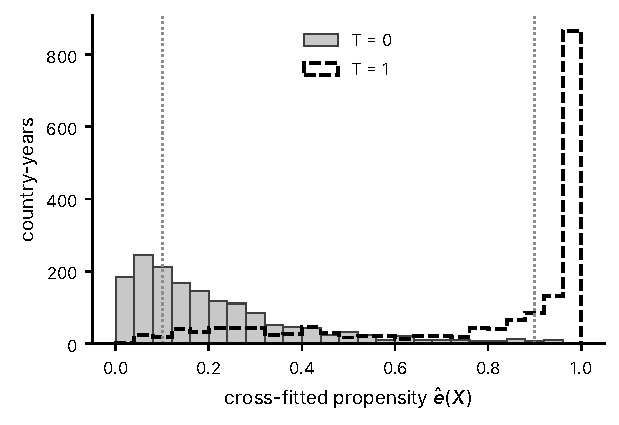
\includegraphics[width=0.75\textwidth]{fig_agri_overlap.pdf}
\caption{Cross-fitted propensity scores for income-adjusted climate-AI capability, by capability
status. Dotted lines mark the trimming bounds 0.1 and 0.9.}
\label{fig:overlap}
\end{figure}

\section{Decile income growth, aggregate growth and costs}\label{app:decile}

This appendix applies EW-DRPL directly to the distributional data. Decile mean income or
consumption comes from the World Bank's Poverty and Inequality Platform. For each country we keep
national surveys of one welfare concept and form spells from consecutive surveys that the
platform flags as comparable and that are at most ten years apart. The outcome is the annualised
log growth of each decile's mean, winsorised at the 1st and 99th percentiles within decile, and
the shock is the mean annual temperature anomaly over the spell. The estimation sample contains
1,334 spells in 124 countries.

Table~\ref{tab:decile} reports the decile-specific resilience effects. The point estimates are more
negative for the poorer deciles, but none is distinguishable from zero, and the average changes sign
across sample splits (from $-4.6$ to $4.1$). The underlying problem is the first stage: the annual
temperature anomaly has no detectable effect on GDP per capita growth in our sample
($-0.10$, SE 0.18; in hot EMDEs $-0.27$, SE 0.46), and spell averages dilute it further. Applied to
country-year GDP growth, the average resilience effect is 0.12 (SE 0.50); in this supplementary
analysis the covariates are measured in the same year as the outcome. Table~\ref{tab:cost}
reports the cost module.

\begin{table}[htbp]
\centering
\caption{Decile income growth: resilience incidence and marginal damages}\label{tab:decile}
\small
\begin{tabular}{lccc}
\toprule
Decile & Resilience effect $E[\Gamma_d]$ & Damage, $T=1$ & Damage, $T=0$ \\
\midrule
1 & -3.11 (2.40) & -0.37 (1.11) & -0.23 (1.13) \\
2 & -2.12 (1.99) & -0.18 (0.73) & 0.27 (0.78) \\
3 & -2.30 (1.92) & -0.23 (0.65) & 0.64 (0.75) \\
4 & -2.04 (1.94) & -0.01 (0.64) & 0.97 (0.68) \\
5 & -1.73 (1.86) & 0.14 (0.59) & 1.12 (0.63) \\
6 & -1.53 (1.85) & 0.21 (0.56) & 1.16 (0.58) \\
7 & -1.39 (1.68) & 0.27 (0.52) & 1.19 (0.57) \\
8 & -0.82 (1.78) & 0.23 (0.53) & 1.07 (0.59) \\
9 & -0.74 (1.74) & -0.00 (0.56) & 1.05 (0.64) \\
10 & 0.02 (1.76) & 0.62 (0.63) & 1.07 (0.82) \\
\midrule Average & -1.58 (1.80) & & \\
\bottomrule
\end{tabular}
\begin{minipage}{0.95\textwidth}\footnotesize\smallskip
\emph{Notes:} 1,334 survey spells in 124 countries (13,340 spell-decile observations). Outcome:
annualised growth of decile mean income or consumption (\%). Shock: mean annual temperature
anomaly over the spell. Capability: income-adjusted climate-AI stock at the start of the spell.
Scores are medians over 20 sample splits; country-clustered SE in parentheses. Damage columns:
mean orthogonal slope score $\psi^*_d$ by capability status.
\end{minipage}
\end{table}


\begin{table}[htbp]
\centering
\caption{The energy and emissions cost of AI capability (double machine learning)}\label{tab:cost}
\small
\resizebox{\textwidth}{!}{%
\begin{tabular}{lcccccc}
\toprule
 & \multicolumn{3}{c}{Log electricity per capita} & \multicolumn{3}{c}{Log CO$_2$ per capita} \\
\cmidrule(lr){2-4}\cmidrule(lr){5-7}
Treatment & Climate-AI stock & AI output & Income residual & Climate-AI stock & AI output & Income residual \\
\midrule
Coefficient (SE) & -0.015 (0.112) & 0.070 (0.060) & -0.046 (0.112) & 0.061 (0.099) & 0.028 (0.056) & 0.054 (0.099) \\
$p$-value & 0.894 & 0.243 & 0.679 & 0.538 & 0.613 & 0.587 \\
High $-$ low renewable share & 0.247 (0.202) & 0.119 (0.098) & 0.423 (0.204) & 0.075 (0.186) & 0.088 (0.108) & 0.196 (0.189) \\
Country-years & 3192 & 3192 & 3192 & 3192 & 3192 & 3192 \\
\bottomrule
\end{tabular}}
\begin{minipage}{0.95\textwidth}\footnotesize\smallskip
\emph{Notes:} Partially linear model with cross-fitted gradient-boosting nuisances (five country
folds) and Mundlak country means of all controls (log GDP per capita, urban share, log population,
internet use, agricultural share, renewable share, baseline temperature, year). 149 countries,
2001--2022. SE clustered by country. Climate-AI stock: $\ln(1+K/\text{pop})$, lagged; AI output:
$\ln(1+$AI works per million$)$, lagged; income residual: capability beyond income (continuous).
\end{minipage}
\end{table}


\section{Additional allocation and solver results}\label{app:allocation}

\begin{table}[htbp]
\centering
\caption{Share of agricultural heat exposure covered at a budget of 37 countries}
\label{tab:coverage}
\small
\begin{tabular}{lrrrr}
\toprule
 & & \multicolumn{3}{c}{Share of sample exposure (\%)}\\
\cmidrule(lr){3-5}
Rule & EMDEs & $\epsilon=0$ & $\epsilon=1$ & $\epsilon=1$\\
 & selected & & Bottom-first & Uniform\\
\midrule
Research-first          &  5 &  3.3 &  1.5 &  0.9 \\
Poorest-first           & 37 & 58.8 & 72.8 & 77.6 \\
Most-agricultural-first & 37 & 63.3 & 78.4 & 83.1 \\
Random (expected)       & 25.3 & 29.4 & 29.4 & 29.4 \\
\bottomrule
\end{tabular}
\begin{minipage}{0.95\textwidth}\footnotesize\smallskip
\emph{Notes.} The sample contains 126 countries, including 86 emerging and developing
economies. The rules rank countries by the country mean of log one
plus lagged climate-AI stock per million people, the country mean of lagged log GDP per capita,
or average agricultural employment share. Columns report
Equation~\eqref{eq:coverage}. At $\epsilon=0$, exposure is proportional to 2023 population
times agricultural employment share times the standard deviation of hottest-month
temperature anomalies. At $\epsilon=1$, the exposure assigned to each income decile
is weighted by the inverse of mean decile income. Bottom-first assigns agricultural
exposure to poorer deciles first; uniform allocates the same exposure fraction to
each decile. The shares use a common slope improvement and can be reproduced with
\texttt{code/31\_application\_agri.py --exposure-shares 0.3}.
\end{minipage}
\end{table}


\begin{table}[htbp]
\centering
\small
\caption{Quota-preserving rules on independent simulated test countries}
\label{tab:swap_simulation}
\begin{tabular}{lrrr}
\toprule
Rule & Gain (MC SE) & Regret & Loss rate (\%) \\
\midrule
\multicolumn{4}{l}{\emph{Moderate overlap}} \\
Exposure baseline & 0.0000 (0.0000) & 0.0373 & 0.0 \\
DR swaps & 0.0055 (0.0012) & 0.0318 & 36.4 \\
Plug-in swaps & 0.0097 (0.0012) & 0.0275 & 30.8 \\
Mean-score swaps & 0.0106 (0.0012) & 0.0266 & 26.8 \\
Robust swaps & 0.0104 (0.0010) & 0.0269 & 27.2 \\
\midrule
\multicolumn{4}{l}{\emph{Weak overlap}} \\
Exposure baseline & 0.0000 (0.0000) & 0.0373 & 0.0 \\
DR swaps & 0.0052 (0.0010) & 0.0320 & 40.6 \\
Plug-in swaps & 0.0078 (0.0011) & 0.0294 & 35.8 \\
Mean-score swaps & 0.0080 (0.0011) & 0.0292 & 36.2 \\
Robust swaps & 0.0096 (0.0009) & 0.0276 & 29.0 \\
\midrule
\multicolumn{4}{l}{\emph{Homogeneous effects}} \\
Exposure baseline & 0.0000 (0.0000) & 0.0000 & 0.0 \\
DR swaps & -0.0219 (0.0009) & 0.0219 & 99.0 \\
Plug-in swaps & -0.0226 (0.0010) & 0.0226 & 97.4 \\
Mean-score swaps & -0.0195 (0.0008) & 0.0195 & 97.8 \\
Robust swaps & -0.0149 (0.0008) & 0.0149 & 87.0 \\
\bottomrule
\end{tabular}

\begin{minipage}{0.9\textwidth}\footnotesize\smallskip
\emph{Notes.} 500 replications per design. Every rule selects 90 of 300 test
countries. Gain is the mean equity-weighted welfare change from the exposure
reference. Regret is relative to the best member of the training-derived library
evaluated with the true test-country benefits. Loss rate is the fraction of
replications with a strictly negative gain, allowing a numerical tolerance.
\end{minipage}
\end{table}

\begin{table}[htbp]
\centering
\small
\caption{Estimated welfare changes relative to exposure-based allocation}
\label{tab:swap_application}
\begin{tabular}{lrr}
\toprule
Rule & Gain [95\% interval] & Replacements \\
\midrule
\multicolumn{3}{l}{\emph{Country folds}} \\
Exposure baseline & 0.000 [0.000, 0.000] & 0 \\
DR swaps & 0.000 [-0.704, 0.750] & 20 \\
Plug-in swaps & -0.069 [-0.558, 0.581] & 19 \\
Mean-score swaps & -0.164 [-0.896, 0.586] & 24 \\
Robust swaps & 0.455 [-0.122, 1.219] & 21 \\
\midrule
\multicolumn{3}{l}{\emph{Region folds}} \\
Exposure baseline & 0.000 [0.000, 0.000] & 0 \\
DR swaps & 0.492 [-0.102, 1.504] & 8 \\
Plug-in swaps & 0.378 [-0.295, 1.405] & 13 \\
Mean-score swaps & 0.451 [-0.224, 1.464] & 7 \\
Robust swaps & 0.065 [-0.184, 0.403] & 14 \\
\bottomrule
\end{tabular}

\begin{minipage}{0.9\textwidth}\footnotesize\smallskip
\emph{Notes.} All rules allocate 37 places across 126 eligible countries. Gain is the
mean difference in equity-weighted welfare using the same orthogonal score with the
propensity clipped at 0.10 for evaluation. Country bootstrap intervals condition on
the learned rules and scores. Replacements count the places allocated to countries
outside the batch-specific reference allocation. The two designs use different
batch definitions and therefore different reference assignments.
\end{minipage}
\end{table}

\begin{table}[htbp]
\centering
\small
\caption{Independent test-country performance of integer portfolios}
\label{tab:ellipsoid_simulation}
\begin{tabular}{lrrr}
\toprule
Rule & Mean gain & Mean regret & Loss rate (\%) \\
\midrule
\multicolumn{4}{l}{\emph{Moderate overlap}} \\
Exposure reference & 0.0000 & 0.0430 & 0.0 \\
Threshold swaps & 0.0109 & 0.0321 & 26.0 \\
Pooled mean & 0.0176 & 0.0254 & 18.5 \\
Ellipsoidal portfolio & 0.0131 & 0.0299 & 5.0 \\
\midrule
\multicolumn{4}{l}{\emph{Weak overlap}} \\
Exposure reference & 0.0000 & 0.0430 & 0.0 \\
Threshold swaps & 0.0076 & 0.0353 & 26.5 \\
Pooled mean & 0.0130 & 0.0300 & 22.5 \\
Ellipsoidal portfolio & 0.0129 & 0.0301 & 3.5 \\
\midrule
\multicolumn{4}{l}{\emph{Homogeneous effects}} \\
Exposure reference & 0.0000 & 0.0000 & 0.0 \\
Threshold swaps & $-0.0130$ & 0.0130 & 80.0 \\
Pooled mean & $-0.0206$ & 0.0206 & 99.0 \\
Ellipsoidal portfolio & $-0.0021$ & 0.0021 & 30.5 \\
\bottomrule
\end{tabular}
\begin{minipage}{0.9\textwidth}\footnotesize\smallskip
\emph{Notes.} 200 replications per design. All rules choose 18 of 60 independent test
countries. Gain uses the true benefits relative to the exposure reference. Regret
uses the unrestricted best portfolio at the same quota. Loss rate is the frequency
of a strictly negative gain. The pooled mean and ellipsoidal portfolios use the
same fitted benefit surface.
\end{minipage}
\end{table}


\begin{table}[htbp]
\centering
\small
\caption{Integer portfolios in held-out agricultural country and region folds}
\label{tab:ellipsoid_application}
\begin{tabular}{lrr}
\toprule
Rule & Gain [95\% interval] & Replacements \\
\midrule
\multicolumn{3}{l}{\emph{Country folds}} \\
Exposure reference & 0.000 [0.000, 0.000] & 0 \\
Threshold swaps & 0.455 [$-0.122$, 1.219] & 21 \\
Pooled mean & 0.054 [$-0.735$, 0.916] & 27 \\
Ellipsoidal portfolio & $-0.271$ [$-0.754$, $-0.009$] & 7 \\
\midrule
\multicolumn{3}{l}{\emph{Region folds}} \\
Exposure reference & 0.000 [0.000, 0.000] & 0 \\
Threshold swaps & 0.065 [$-0.184$, 0.403] & 14 \\
Pooled mean & $-0.048$ [$-1.019$, 1.136] & 25 \\
Ellipsoidal portfolio & 0.000 [0.000, 0.000] & 0 \\
\bottomrule
\end{tabular}
\begin{minipage}{0.9\textwidth}\footnotesize\smallskip
\emph{Notes.} 37 places across 126 countries in each design. Gains use the same
held-out DR score with propensity clipping at 0.10. Conditional intervals resample
country contributions while holding the fits and portfolios fixed. A zero gain and
zero-width interval result mechanically when the portfolio is the reference.
\end{minipage}
\end{table}


\begin{table}[htbp]
\centering
\small
\caption{Exchange-grid and integer cutting-plane certificates}
\label{tab:exchange_grid}
\begin{tabular}{lrrr}
\toprule
& \multicolumn{3}{c}{Certified / total instances}\\
\cmidrule(lr){2-4}
Design & Exchange grid & Grid without tilt & Cutting planes\\
\midrule
One-factor lattice & 16/16 & 16/16 & 16/16\\
Two-factor lattice & 16/16 & 16/16 & 16/16\\
Six continuous factors & 0/16 & 0/16 & 16/16\\
Agriculture country folds & 1/5 & 0/5 & 5/5\\
Agriculture region folds & 5/7 & 4/7 & 7/7\\
\bottomrule
\end{tabular}
\begin{minipage}{0.9\textwidth}\footnotesize\smallskip
\emph{Notes.} A certificate has upper-minus-lower bound at most $10^{-5}$ in
total-gain units. Median runtime in the one-factor lattice is 1.1 milliseconds
for the exchange grid and 7.3 for cutting planes. On the two-factor lattice the
corresponding values are 6.8 and 21.2 milliseconds. Timings are specific to this
benchmark and machine.
\end{minipage}
\end{table}



\end{document}
